\chapter{\uppercase{Research Directions} \label{chapter:05}}


\section{Alternative Experimental Designs}

In this section we return to the nonlinear examples presented in the previous chapter and address the choices made in experimental design.
We demonstrate that the decisions made regarding measurement equipment and/or location have an impact on the reduction of uncertainty and accuracy of the MUD point.

We demonstrate the use of the WME map defined in \eqref{eq:qoi_WME_fixed_data} on a problem incorporating a single stream of time-series data for a first-order ODE problem.

\subsection{ODE Example}
Consider an exponential decay problem with uncertain decay rate:

$$
\begin{cases}
\frac{\partial u}{\partial t} & = \param u(t) \\ u(0) &= 0.75
\end{cases}
$$

The solution is described by
\begin{equation}
  u(t) = u_0\exp(-\param t), \; u_0 = 0.75 ,
\end{equation}
where we consider $t \in [0, 3]$, allowing measurements to begin for $t\geq 1$.
\begin{figure}[htbp]
  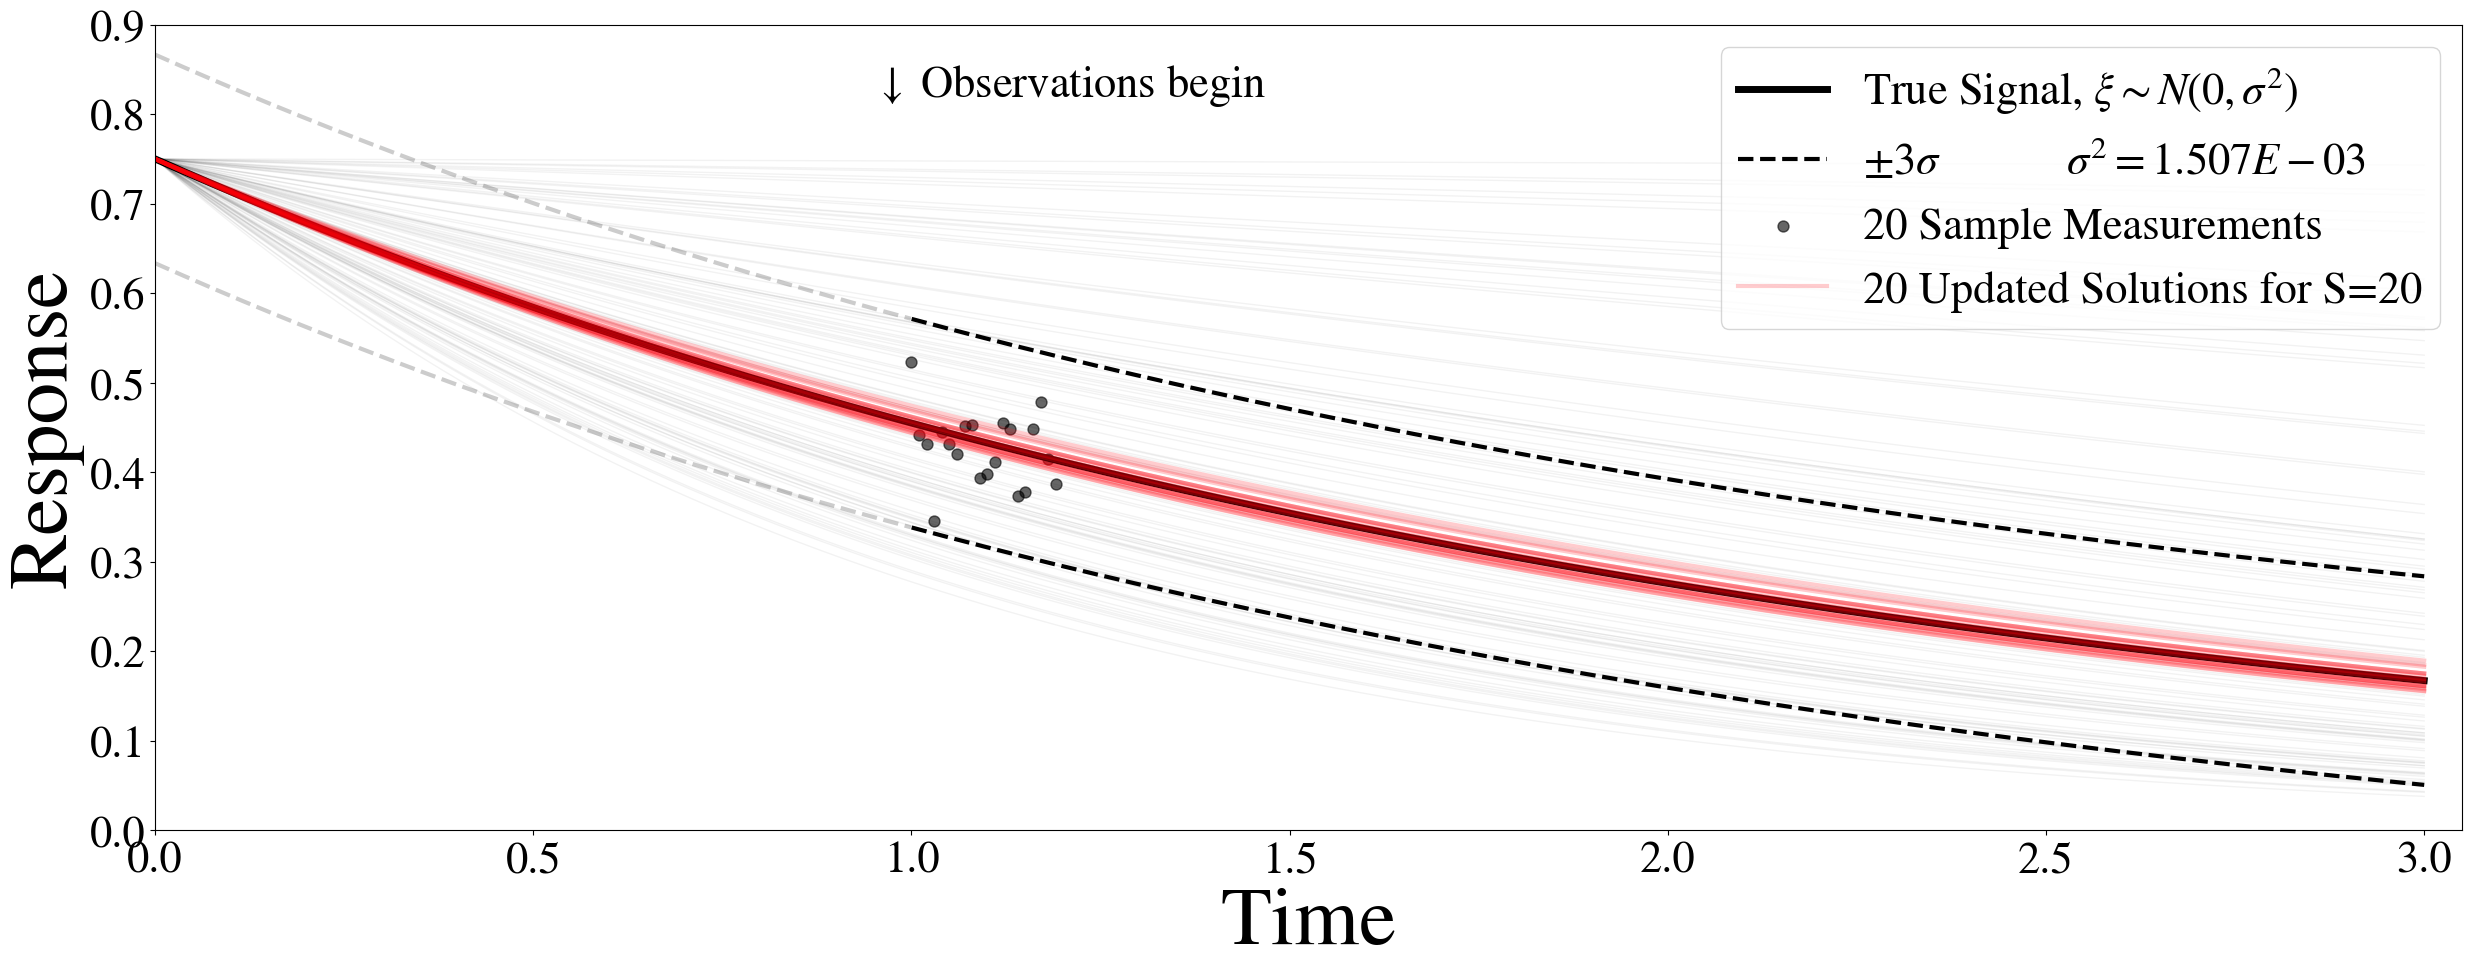
\includegraphics[width=\linewidth]{figures/ode/ode_20_reference_solution}
  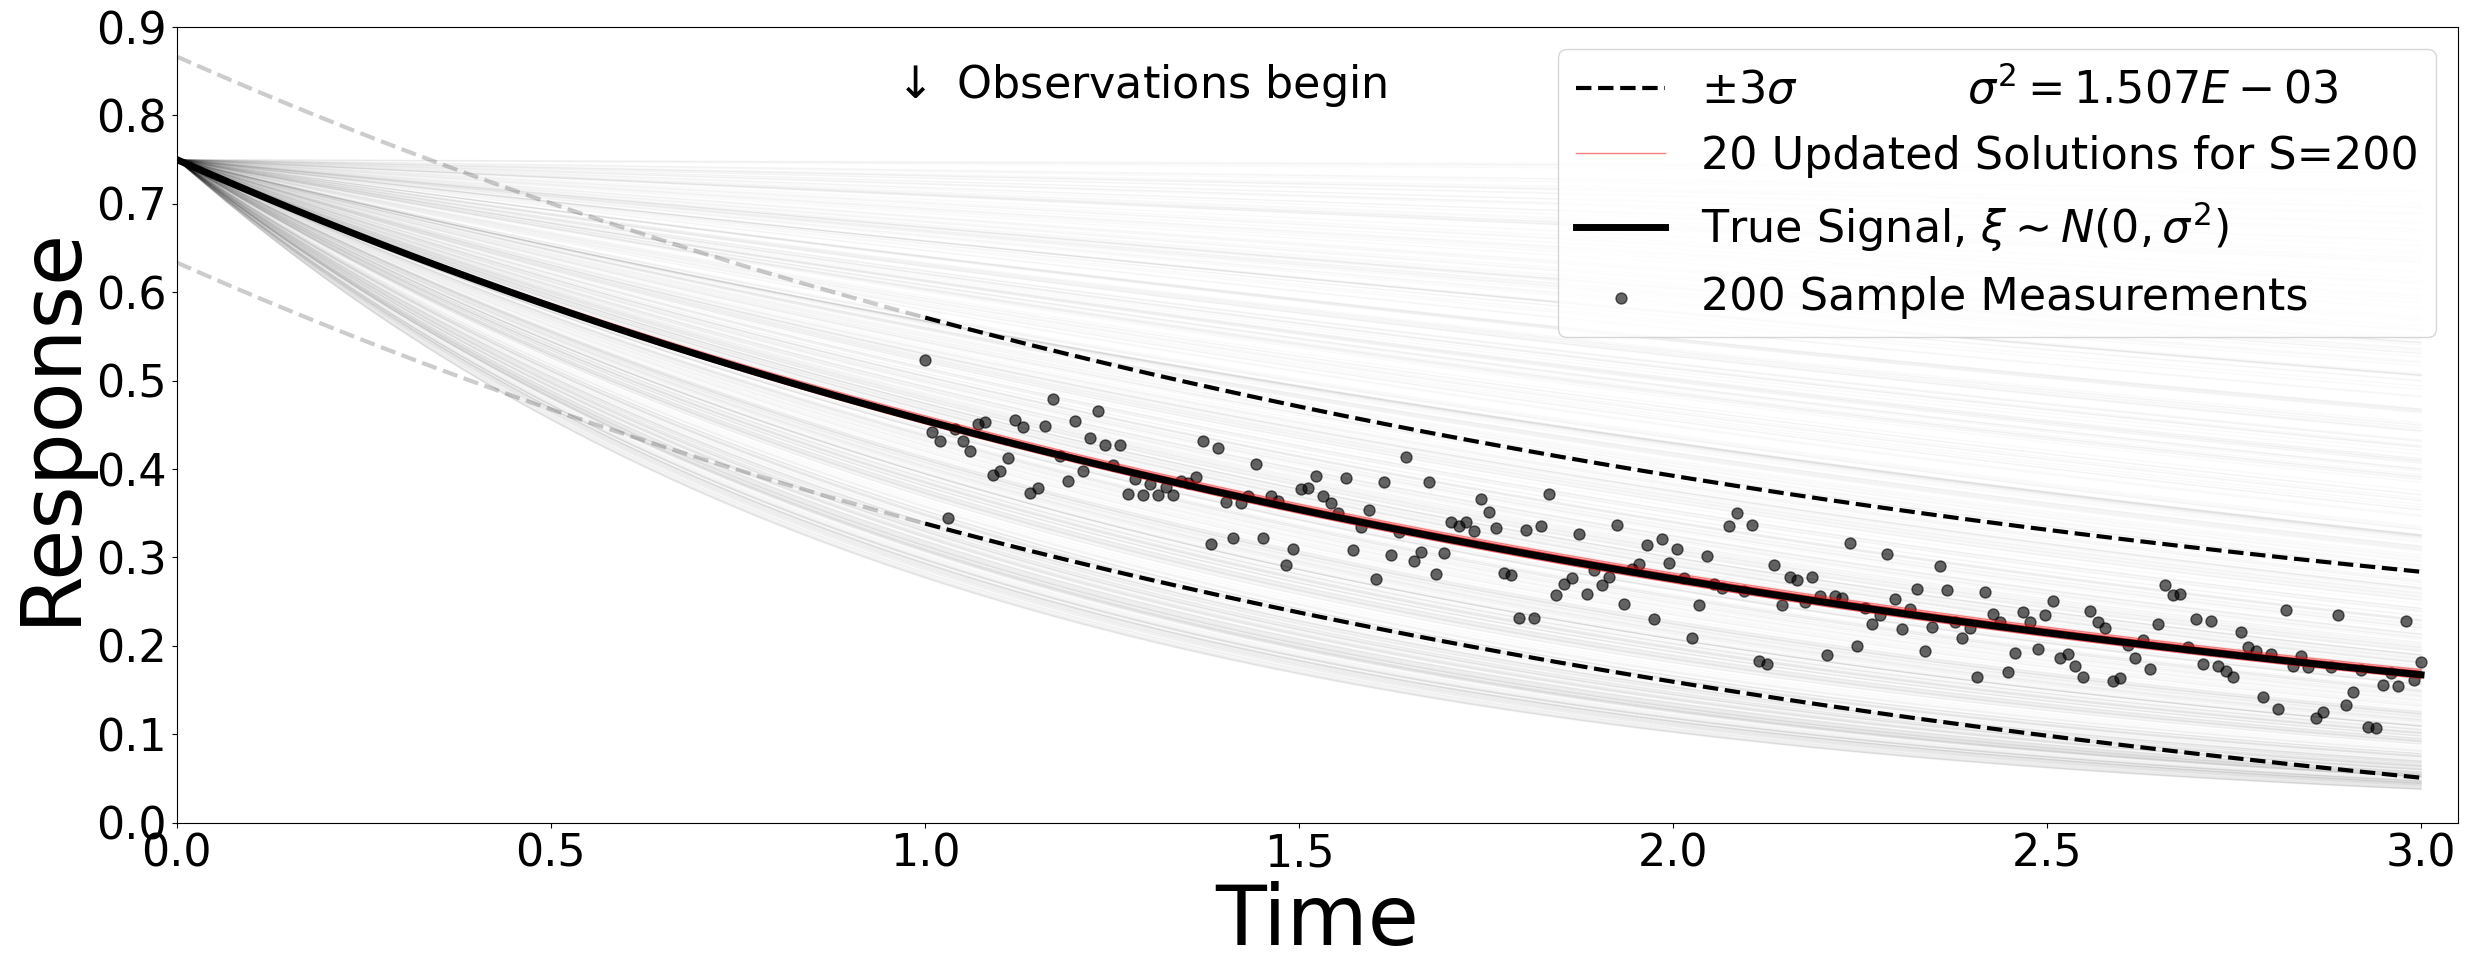
\includegraphics[width=\linewidth]{figures/ode/ode_200_reference_solution}
  \caption{Time series response for exponential decay with markers for the assumed error intervals for observations.
  Measurements are taken over the time interval $(1,3)$.
  Five-hundred draws from $\pi_\text{init}$ are used to generate sample responses and are shown in gray.
  (Top): Twenty updated solution (the results of the repeated trials) for $S=25$ are plotted in blue, and capture the true signal.
  (Bottom): The solution for using all $S=200$ measurements available that were taken over the observation window.
  }
  \label{fig:ode-reference}
\end{figure}

We consider a uniform prior over $\param \in \Lambda = (0, 1)$ to represent our uncertainty about the decay rate.
Measurements are simulated over the interval $t \in [1,3]$ for observations from a $100$Hz sensor, and are perturbed (as outlined in \ref{subsec:example-setup}).
An example of this setup is shown in Figure~\ref{fig:ode-reference}, with the solid line representing the ``true'' signal obtained by evaluating the solution for $\param = 0.5$, and an example of possible measurements shown as perturbed points around it.


\begin{figure}[htbp]
  \centering
  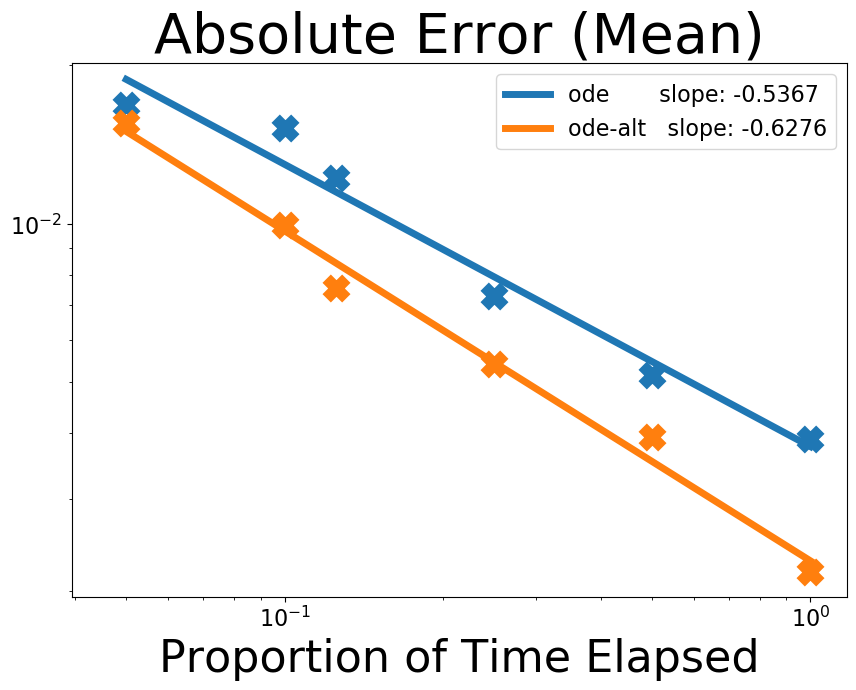
\includegraphics[width=0.475\linewidth]{figures/ode/ode_convergence_mud_obs_mean}
  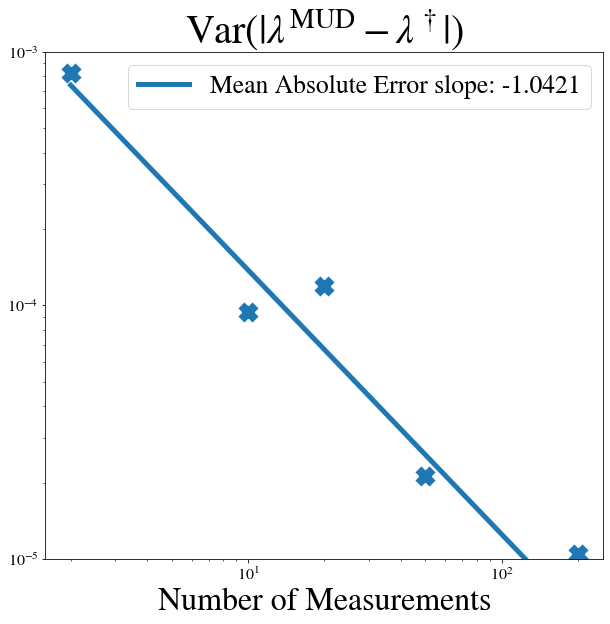
\includegraphics[width=0.475\linewidth]{figures/ode/ode_convergence_mud_obs_var}

  \caption{Convergence of the MUD point given $N=1E4$ model evaluations for increasing numbers of observations for randomly placed sensors.
  Convergence rates are estimated using first-order linear regressions in $\text{log}_{10}$-space.
  $100$Hz equipment demonstrates a reduction of uncertainty and improvement in precision as $S$ increases towards $200$.
  We observe the same rates of convergence for the alternative equipment and note the (slightly) lower overall error for equal numbers of measurements ($S=200$ corresponding to $t\in (1,2)$ in this formulation).
  }
  \label{fig:ode-convergence-obs}
\end{figure}
We sequentially incorporate $S=5, 10, 15, 20, 25, 50, 100, \text{ and } 200$ measurements and study the error in our estimate of $\param_\text{ref}$.
In the top half of Figure~\ref{fig:ode-convergence-obs}, we can observe that as more measurements are incorporated to the solution of the inverse problem, both precision and accuracy are improved.



To achieve higher precision in the estimate of the MUD point, one can use more precise measurement equipment.
Rather than a tolerance of one decimal place, we consider choices of $\tau = 0.1, 0.05, 0.01, 0.005, \text{ and } 0.001$ for $\mathbb{P}( \abs{\xi} < \tau ) = 99\%$ to select our $\sigma$ in our normal additive noise.
In Figure~\ref{fig:ode-convergence-std}, we study the absolute error's mean and variance as our measurement equipment gets more precise.


\begin{figure}[htbp]
  \centering
  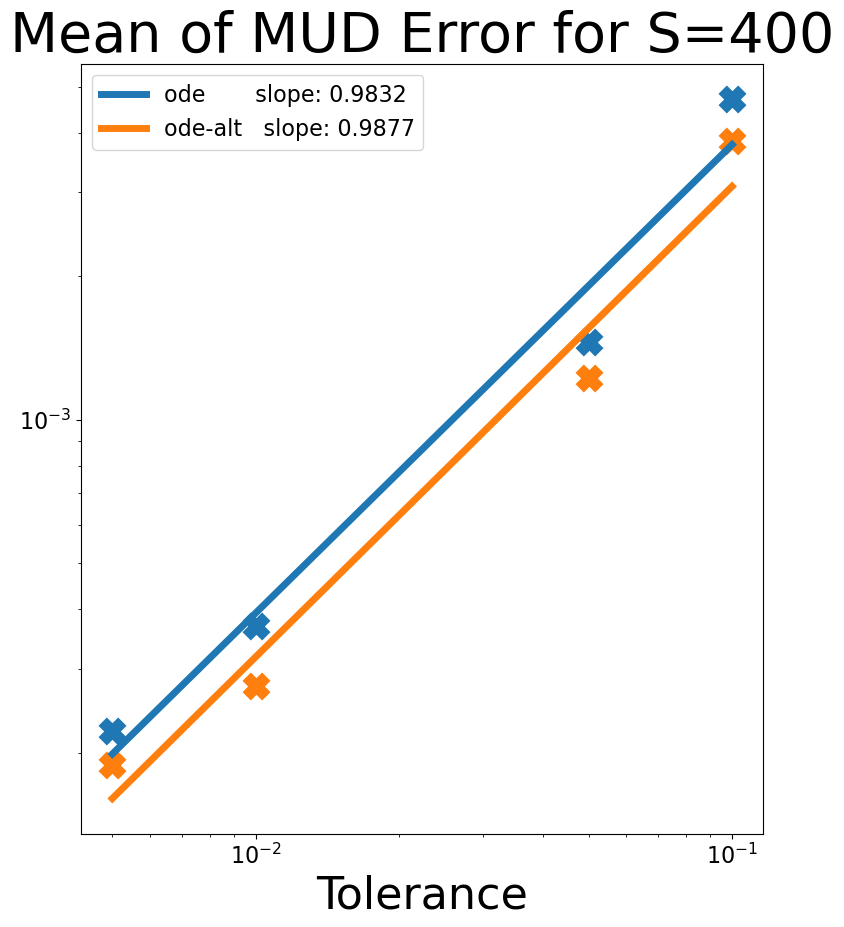
\includegraphics[width=0.475\linewidth]{figures/ode/ode_convergence_mud_std_mean}
  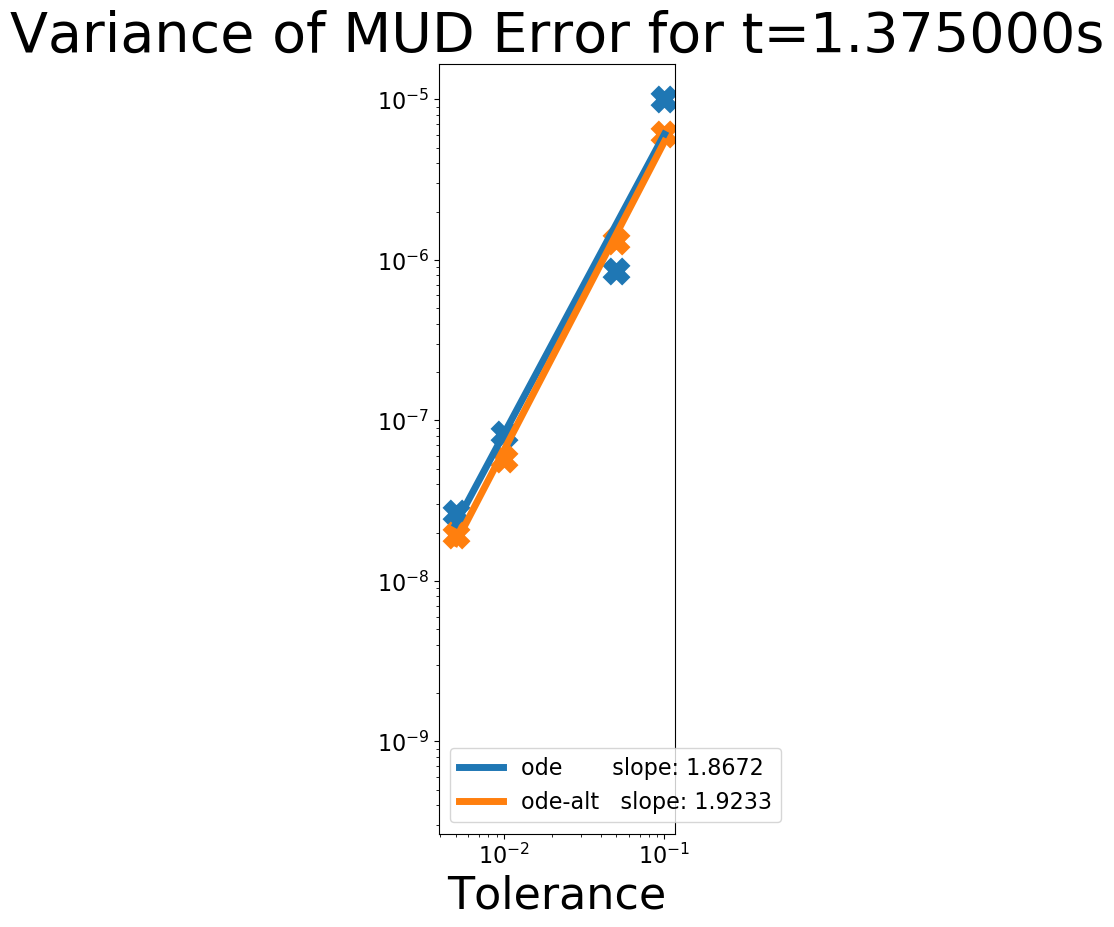
\includegraphics[width=0.475\linewidth]{figures/ode/ode_convergence_mud_std_var}

  \caption{Convergence of the MUD point given $N=1E4$ model evaluations for different precisions of observations for randomly placed sensors, incorporating $S=25$ measurements.
  As more exact measurements are incorporated, the accuracy and precision of the MUD solution improves, convergence rates are estimated with regression, and appear to be unaffected .
  }
  \label{fig:ode-convergence-std}
\end{figure}

TK - say more here.


%%%%%%%%%%%%%%%%%%%%%%%%%%%%%%%%%%%%%%%%%%%%%%%%%%%%%%%%%%%%%%%%%%%%
%%%%%%%%%%%%%%%%%%%%%%%%%%%%%%%%%%%%%%%%%%%%%%%%%%%%%%%%%%%%%%%%%%%%
\subsubsection{Different Measurement Equipment}

We consider the same problem as in the previous section to address the following question: what would happen if our measurement equipment were able to capture twice as many observations?
Instead of using equipment that operates at $100$Hz, we take $200$ measurements every second, resulting in 400 equispaced observations for $t \in (1,3)$.
All other choices involved in the experiment (assumed equipment tolerance, number of trials, parameter samples) are kept the same.

\begin{figure}[htbp]
  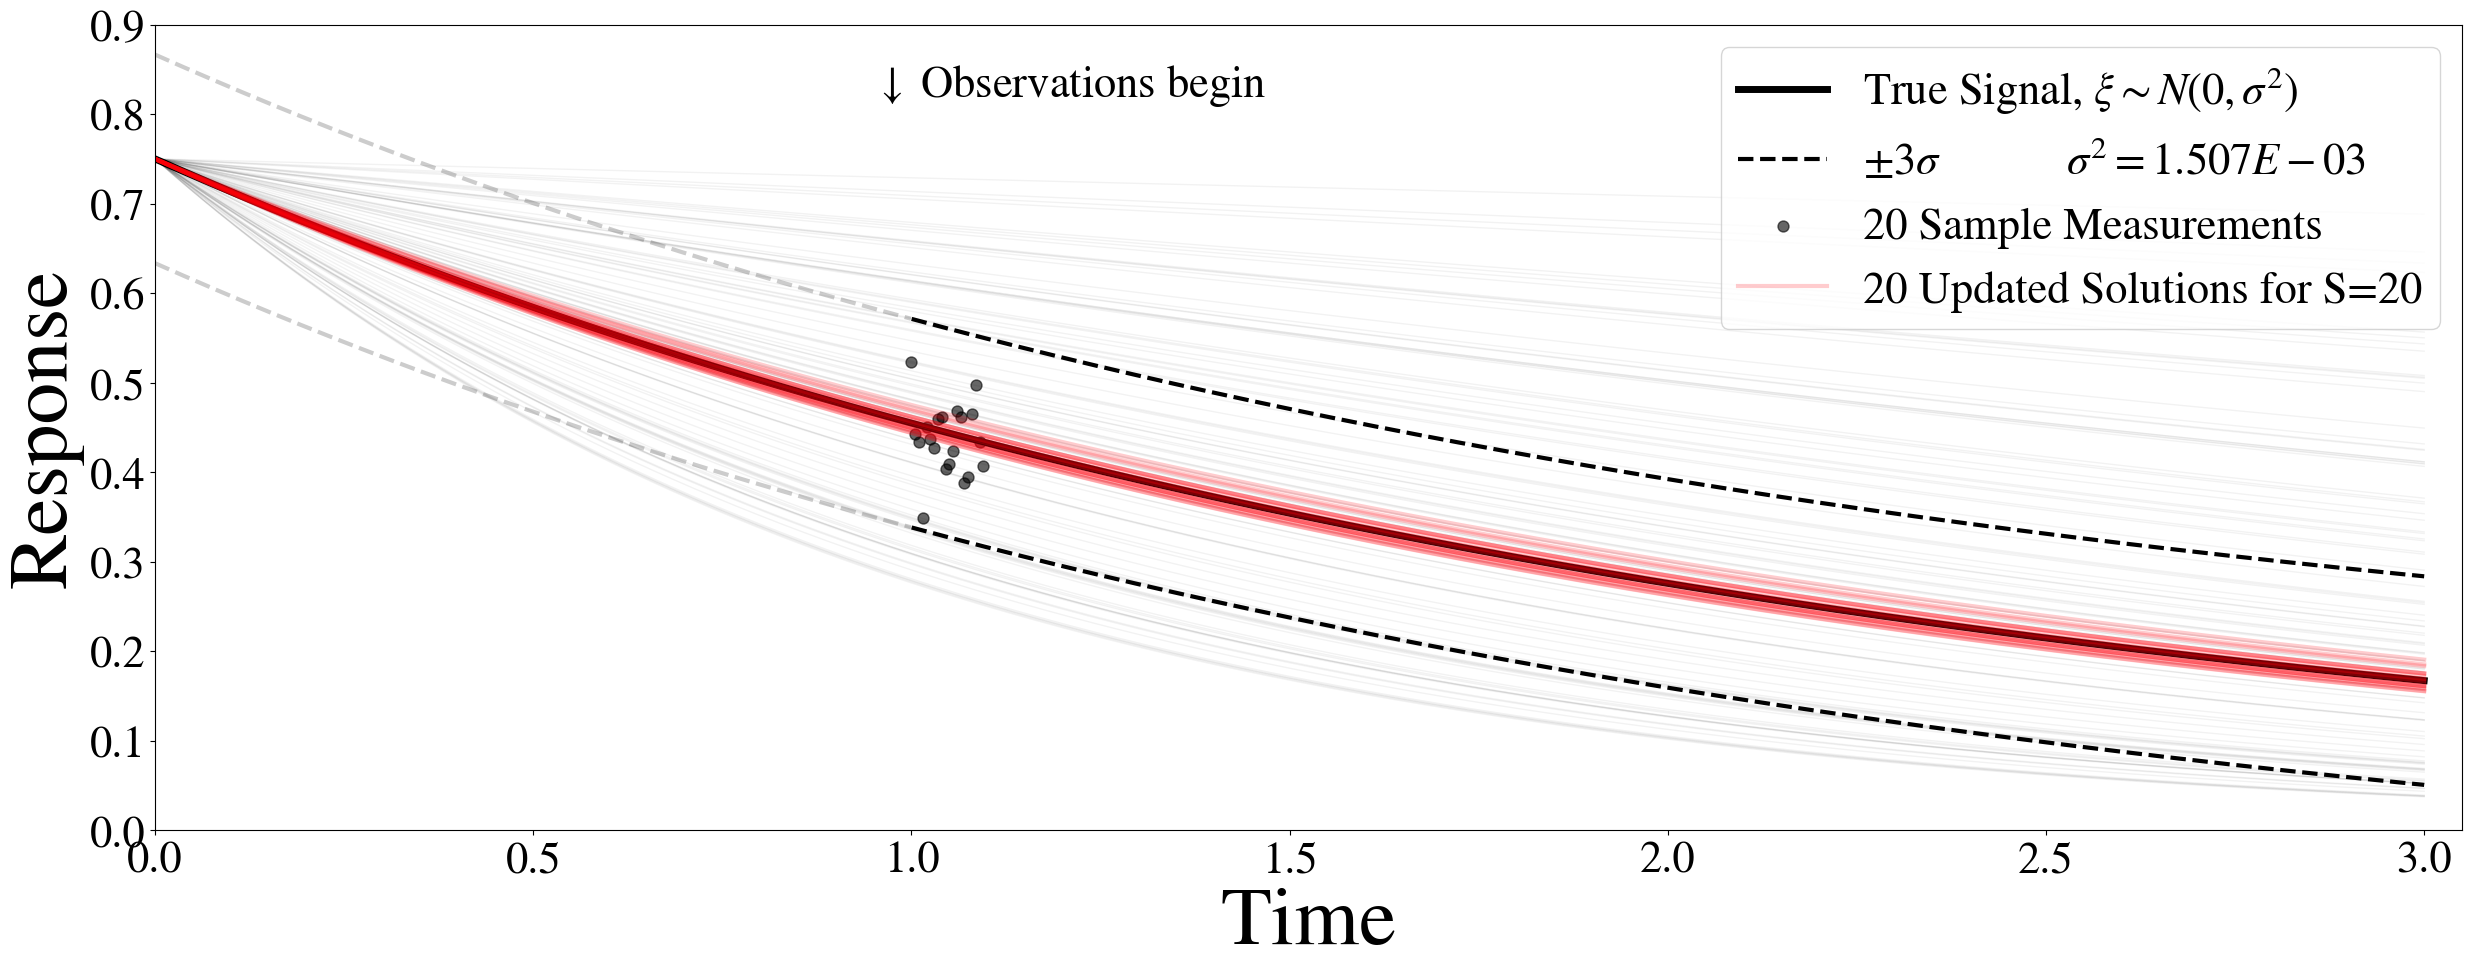
\includegraphics[width=\linewidth]{figures/ode/ode-alt_20_reference_solution}
  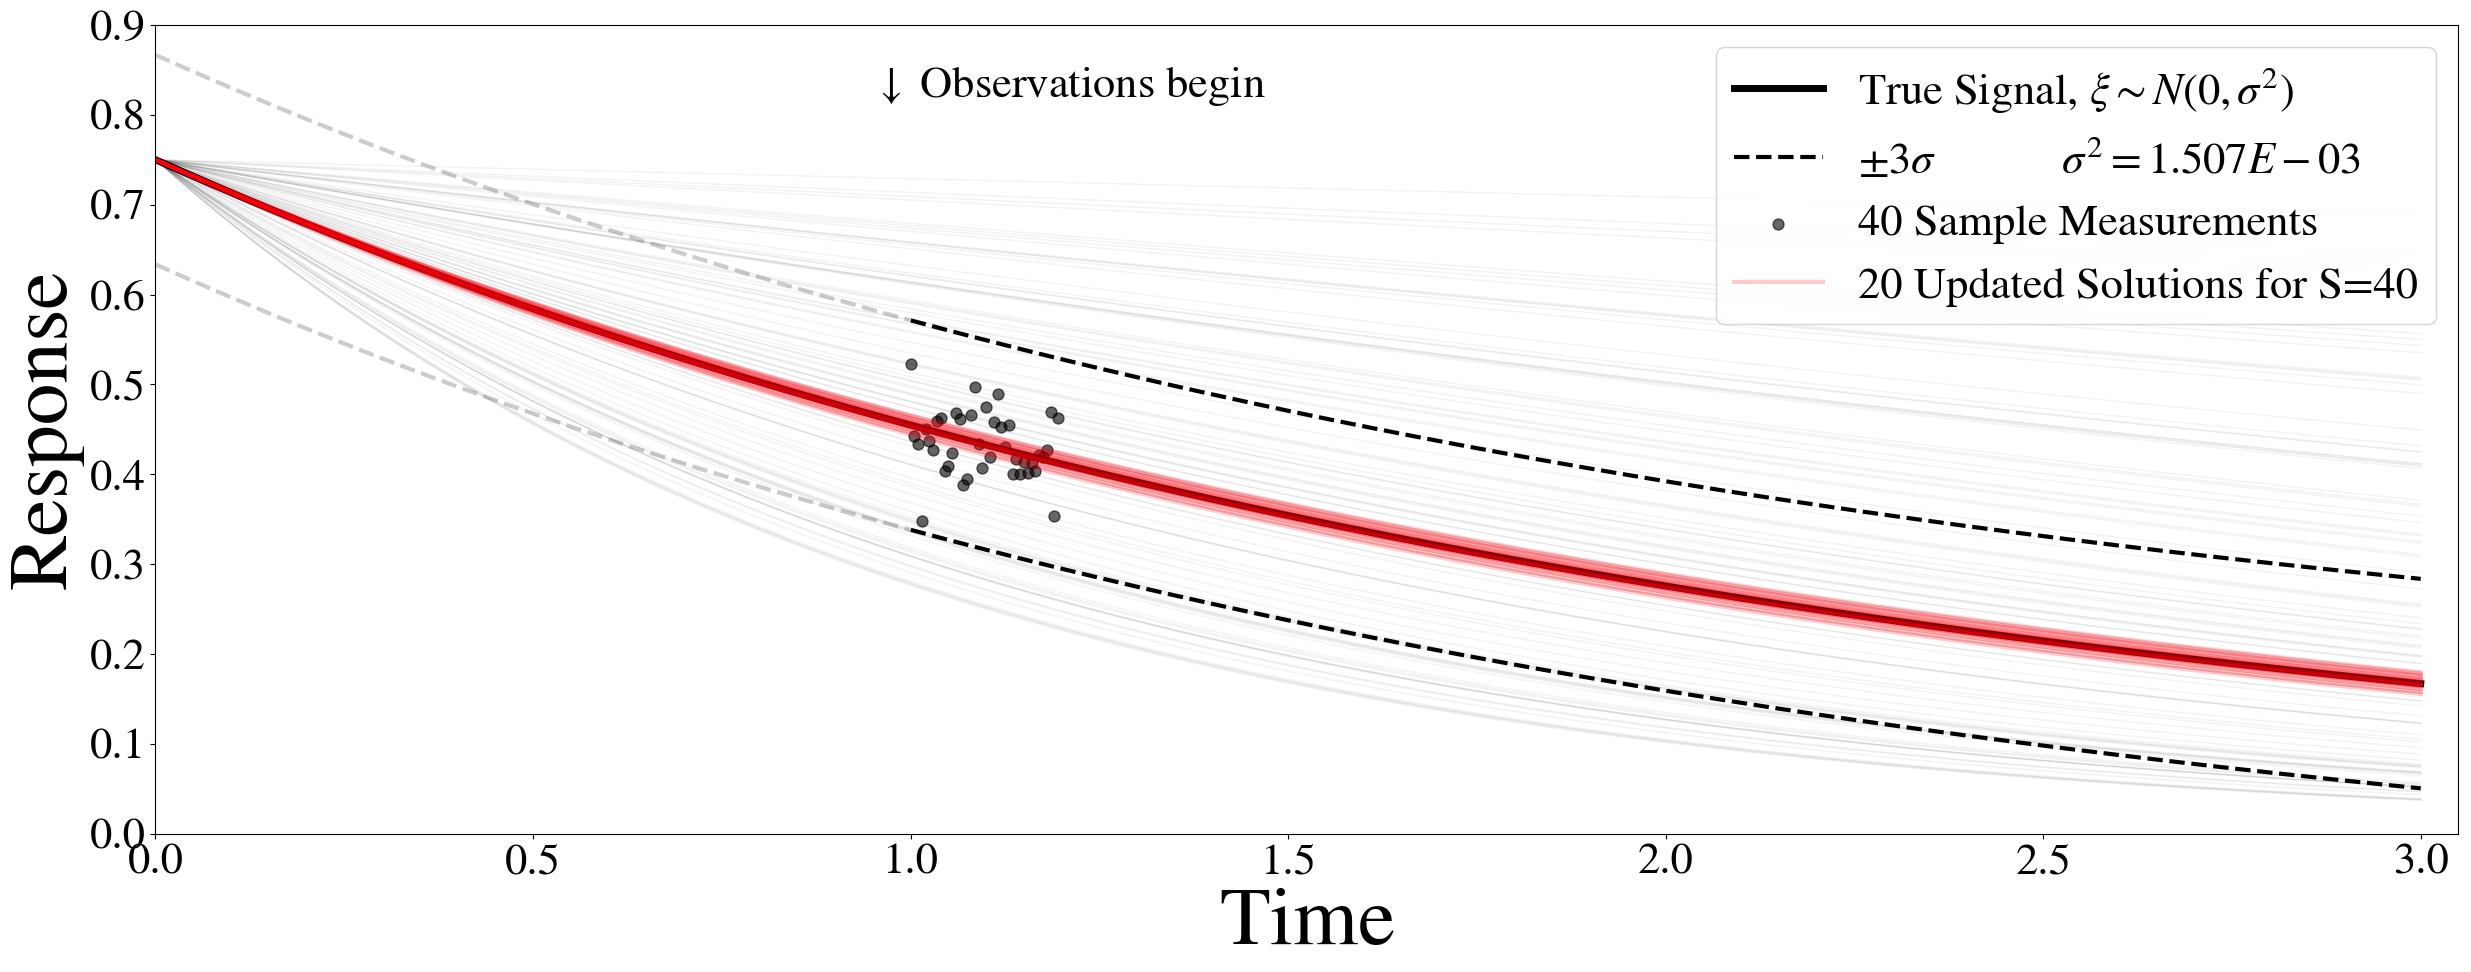
\includegraphics[width=\linewidth]{figures/ode/ode-alt_40_reference_solution}
  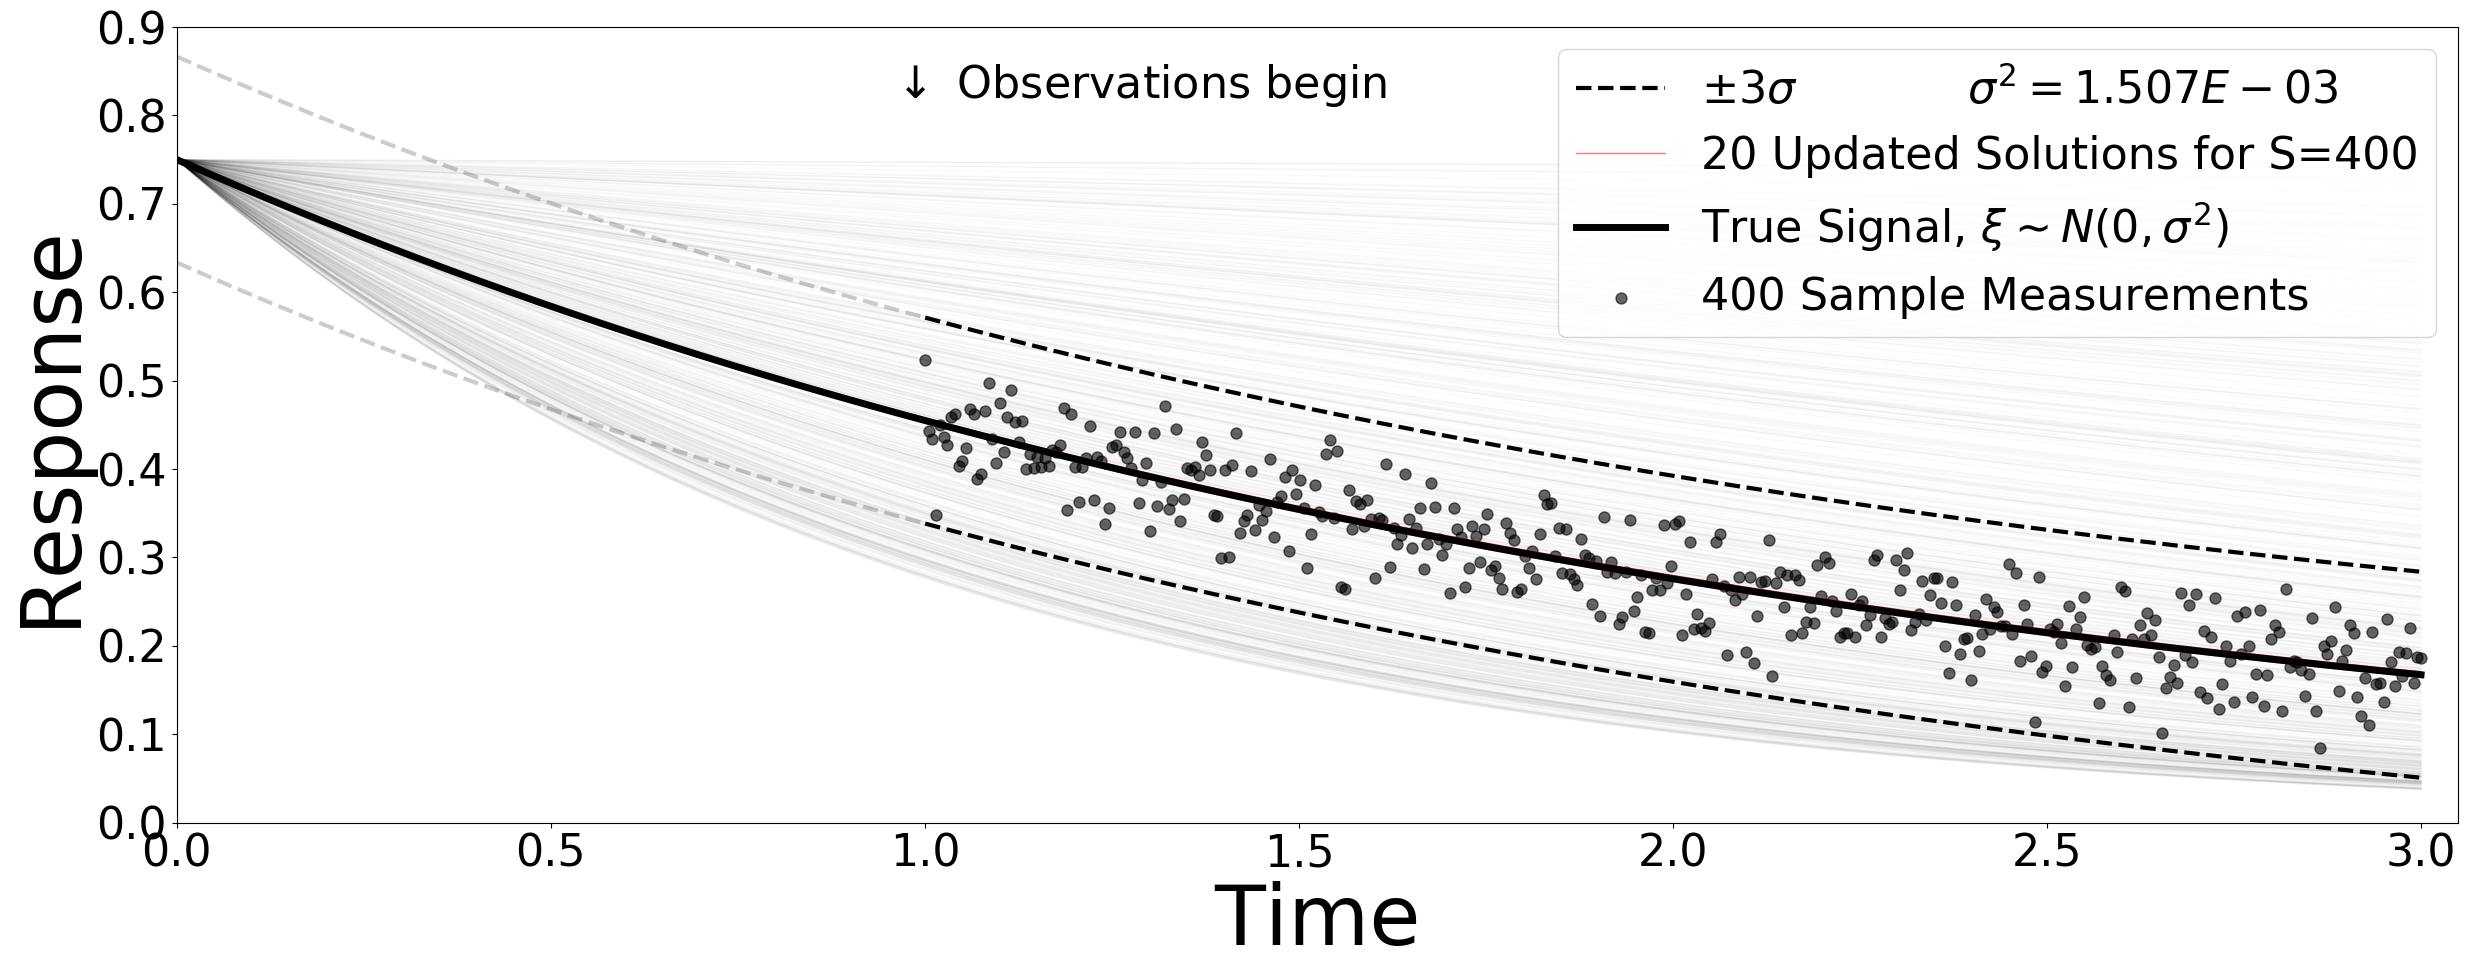
\includegraphics[width=\linewidth]{figures/ode/ode-alt_400_reference_solution}
  \caption{The associated signals for the alternative measurement equipment that operates at twice the frequency.
  The true signal is well-recovered.
  (Top): First twenty-five measurements.
  (Middle): Observations made over the same time interval as in the top half of Figure~\ref{fig:ode-reference}, corresponding to $S=50$.
  (Bottom): The entire observation window is used to solve the problem. Most of the twenty trials appear to identify the same point $\param_i$ ($1\leq i \leq N$), in the sampled parameter set.
  }
  \label{fig:ode-alt-reference}
\end{figure}
First, we note that in Figure~\ref{fig:ode-alt-reference} the predicted signals incorporating the same number of measurements look indistinguishable for $S=25$ compared to those in Figure~\ref{fig:ode-reference}.



We solve the problem for the same choices of $S$ (with the addition of $S=400$, and show the resulting error plots for convergence in the right half of Figures~\ref{fig:ode-convergence-obs} and \ref{fig:ode-convergence-std}.
The convergence rates appear to be the same and reduction in uncertainty is almost negligible.
However, we note that in the alternative setup, for an equal number of measurements, the time elapsed is half of that in the original.
This implies that we can achieve similar results with a shorter observational window by using equipment that allows for faster observations.

We have shown that the Data--Consistent approach to solving parameter identification problems manages to generalize to problems involving time-series data from a single Quantity of Interest.
We now turn our attention to an example where instead of temporal measurements, we incorporate spatial ones to solve another parameter identification problem.
% \vfill
% \pagebreak



%%%%%%%%%%%%%%%%%%%%%%%%%%%%%%%%%%%%%%%%%%%%%%%%%%%%%%%%%%%%%%%%%%%%
%%%%%%%%%%%%%%%%%%%%%%%%%%%%%%%%%%%%%%%%%%%%%%%%%%%%%%%%%%%%%%%%%%%%

%%%%%%%%%%%%%%%%%%%%%%%%%%%%%%%%%%%%%%%%%%%%%%%%%%%%%%%%%%%%%%%%%%%%
%%%%%%%%%%%%%%%%%%%%%%%%%%%%%%%%%%%%%%%%%%%%%%%%%%%%%%%%%%%%%%%%%%%%
\subsection{Elliptic PDE Example}\label{subsec:pde-example}

Consider the following Poisson problem defined on a unit domain:
\begin{equation}\label{eq:pde-equation}
\begin{cases}
\hfill -\nabla \cdot \nabla u &= f \quad\text{on } \Omega \\
\hfill u &= 0 \quad\text{ on } \Gamma_T \cup \Gamma_B \\
\hfill \frac{\partial u}{\partial \mathbf{n}} &= g(x,\param) \quad\text{ on } \Gamma_L \\
\hfill \frac{\partial u}{\partial \mathbf{n}} &= 0 \quad\text{ on } \Gamma_R
\end{cases}
\end{equation}
where $(x_1, x_2) \in \Omega = (0,1)^2$, $\Gamma_T$ is the top, $\Gamma_B$ is the bottom, $\Gamma_L$ and $\Gamma_R$ left and right, respectively.
$\frac{\partial u}{\partial \mathbf{n}}$ denotes the outward normal direction.

\begin{figure}[htbp]
\centering
  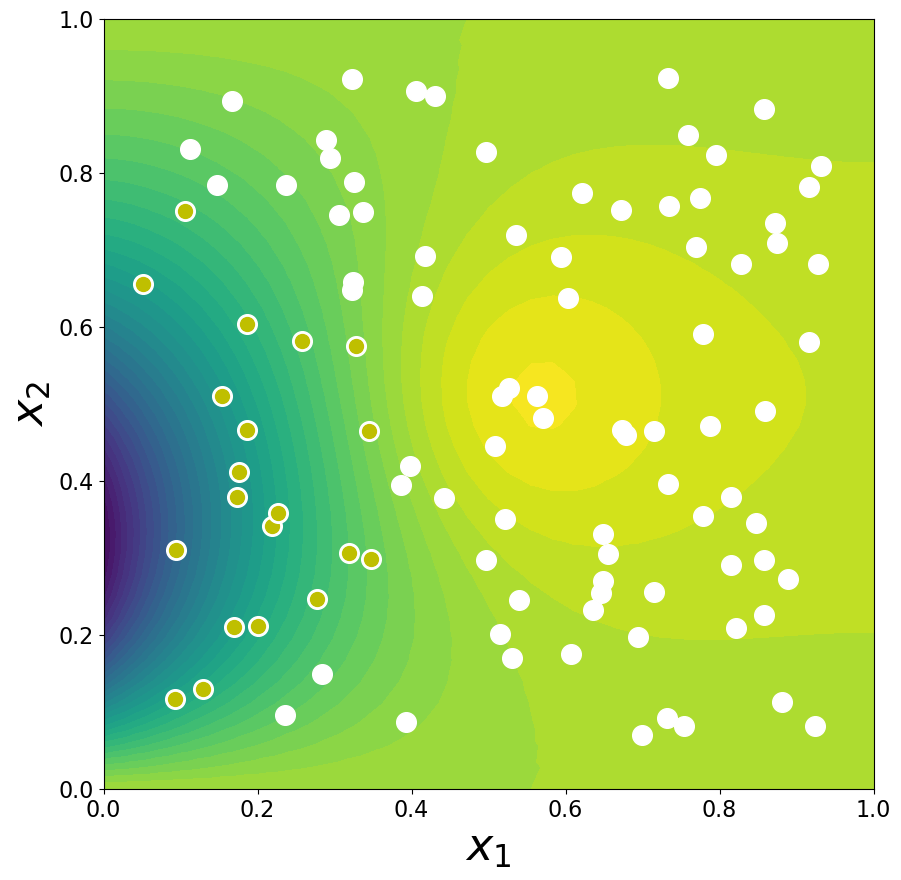
\includegraphics[width=0.475\linewidth]{figures/pde/pde_reference_solution}
  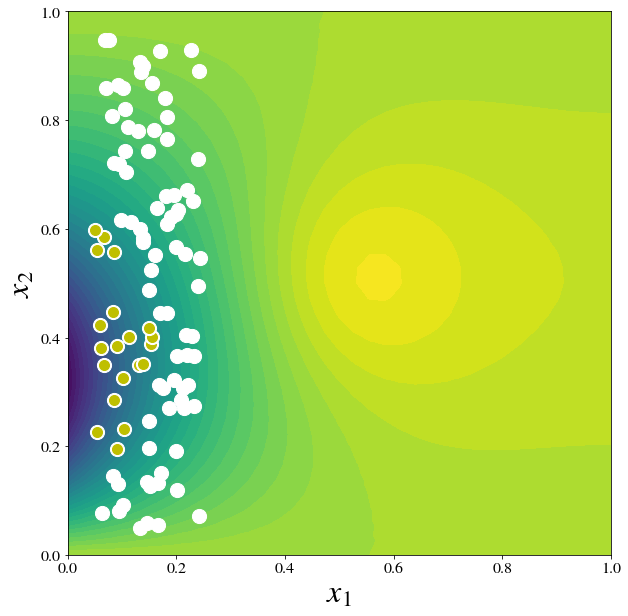
\includegraphics[width=0.475\linewidth]{figures/pde/pde-alt_reference_solution}
\caption{The function response surface for $u$ solving \eqref{eq:pde-equation} with $S=100$ measurement locations highlighted in white.
The twenty most sensitive locations are highlighted in yellow.
(Top): Uninformed sensor placement, where the most sensitive points  appear to cluster around the center of the  left boundary.
This observation is used to inform a better placement.
(Bottom): An alternative random arrangement of $S=100$ measurement locations.
}
\label{fig:pde-ref-solution}
\end{figure}
We select $g=\param \sin(\pi x_2)$, and show the response surface for our given choice of $\param = 3$ in Figure~\ref{fig:pde-ref-solution}.
Our initial density is chosen to be uniform over the interval $\Lambda = (1,5)$.
$f$ is chosen to be $10\exp\{-\frac{(x_1-0.5)^2 + (x_2 - 0.5)^2}{0.02}\}$



One could place a regular grid of sensors in the interior of $\Omega$ to simulate a sensor array of some sort.
However, observe that the response surfaces shown in Figure~\ref{fig:pde-ref-solution} exhibit vertical symmetry about the line $x_1=0.5$ (as a result of our choice of $g$).
We are interested in demonstrating the impact of incorporating more measurements, which poses a problem for this particular experimental design since it will heavily rely on the way in which the sensor grid is indexed.
For example, if the first half of indexed sensors corresponded to the bottom half of $\Omega$, the incorporation of the second half will be equivalent to having repeated observations.
Moreover, since the left-side of $\Omega$ is more sensitive to changes in $\param$ than the right, indexing in a serpentine manner will lead to sharper declines in uncertainty whenever a sensor from a different row gets incorporated.
To avoid these problems, we instead simulate the sensors as being placed randomly in the interior so that index-dependence becomes irrelevant and  probability theory ensures the lack of truly redundant measurement locations.

%%%%%%%%%%%%%%%%%%%%%%%%%%%%%%%%%%%%%%%%%%%%%%%%%%%%%%%%%%%%%%%%%%%%
%%%%%%%%%%%%%%%%%%%%%%%%%%%%%%%%%%%%%%%%%%%%%%%%%%%%%%%%%%%%%%%%%%%%
\subsubsection{Uninformed Sensor Placement}

We consider a selection of $S=1000$ measurement locations in the interior of the response surface chosen by sampling a uniform density over the set $(0.05, 0.95)^2 \subset \Omega$.
In Figure~\ref{fig:pde-sensitivity}, we plot the data generated by each simulated sensor location, and observe that some measurements are more sensitive in others.
The majority of measurements exhibit almost no sensitivity to changes in $\param$, visually represented by near-horizontal lines.
However, some of the sensors have steep slopes, indicating higher sensitivity to the unknown parameter.
To generate convergence plots, we use all thousand available measurements but solve the problem repeatedly for $S = 5, 10, 15, 20, 25, 50, 100, 250, 500, \text{ and } 1000$.


\begin{figure}[htbp]
\centering
  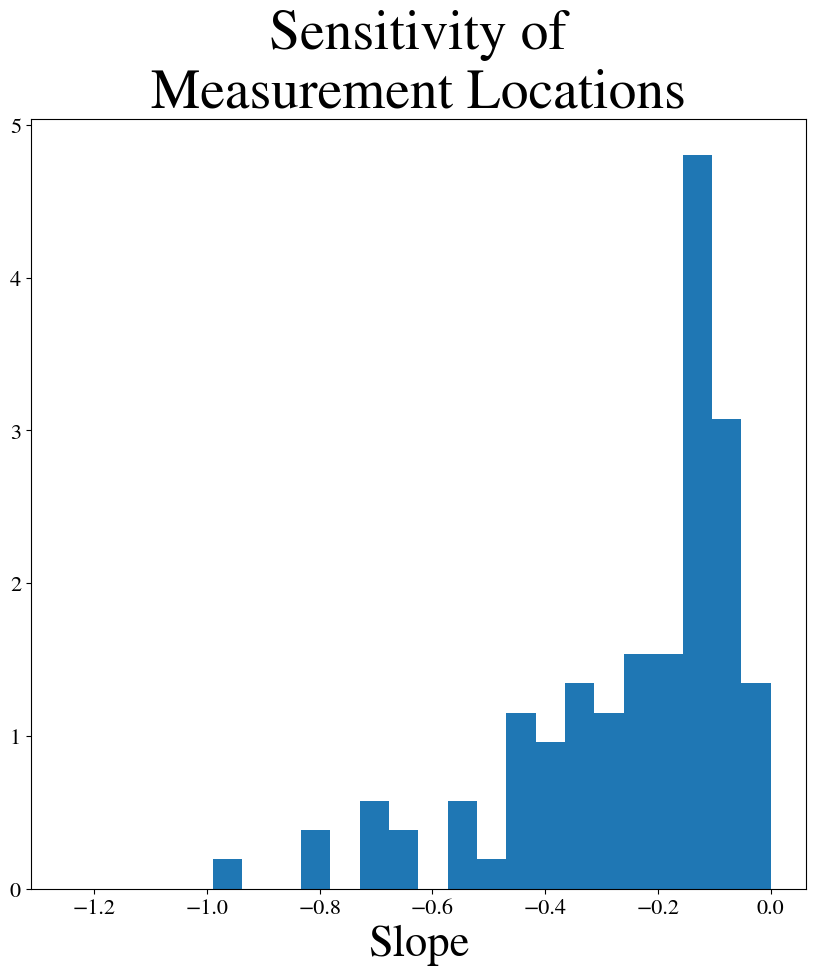
\includegraphics[width=0.35\linewidth]{figures/pde/pde_sensitivity_qoi}
  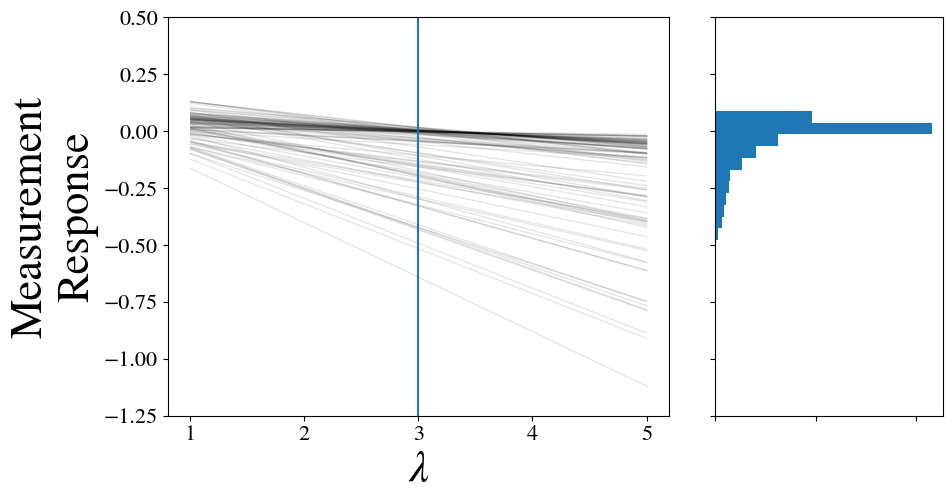
\includegraphics[width=0.6\linewidth]{figures/pde/pde_qoi_response}
  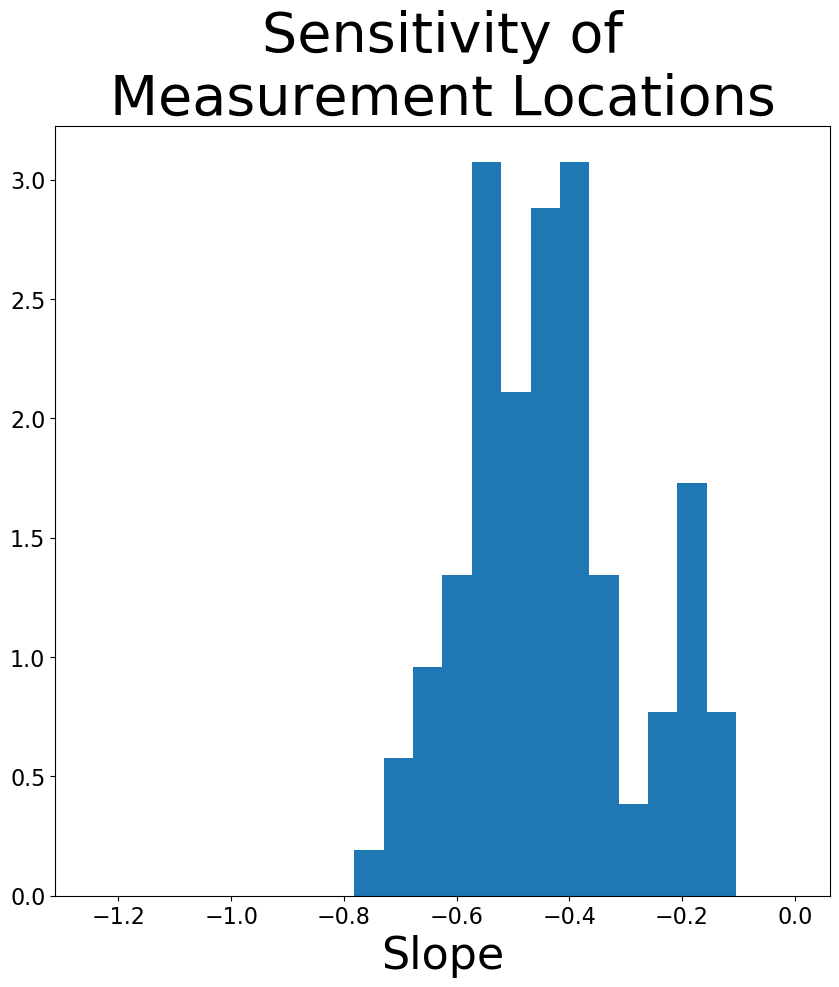
\includegraphics[width=0.35\linewidth]{figures/pde/pde-alt_sensitivity_qoi}
  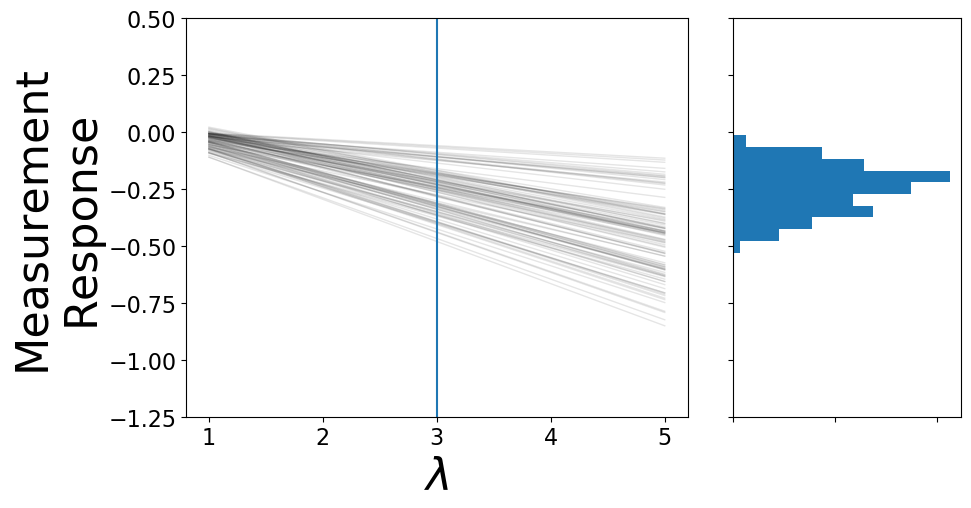
\includegraphics[width=0.6\linewidth]{figures/pde/pde-alt_qoi_response}
  \caption{We plot the values of the response surface evaluated at all $S=1000$ random measurement locations.
  The histogram depicts the measurement values of the response surface evaluated at the true parameter value $\param_\text{ref}=3$.
  (Left): Sensitivity of measurements as a function of $\param$, the scaling for the left boundary condition function.
  (Right): Since the response at each measurement location is linear with respect to $\param$, we compute the slopes for all $S=1000$ sensors and show the associated histogram.
  (Top): Uninformed sensor placement. Observe that most locations are insensitive to changes in $\param$. The ratio of most to least sensitive slopes exceeds 50.
  (Bottom): Informed sensor placement. The informed sensors have much less variability in their respective sensitivities (ratio closer to 10).
  }
\label{fig:pde-sensitivity}
\end{figure}



We are interested in knowing how the uncertainty around the parameter estimate (the MUD point) changes as we incorporate more (noisy) data.
Consider the plots in the left-half of Figure~\ref{fig:pde-convergence-obs}, which demonstrates the impact of increasing $S$ on our ability to resolve $\param_\text{ref}$.


\begin{figure}[htbp]
  \centering
  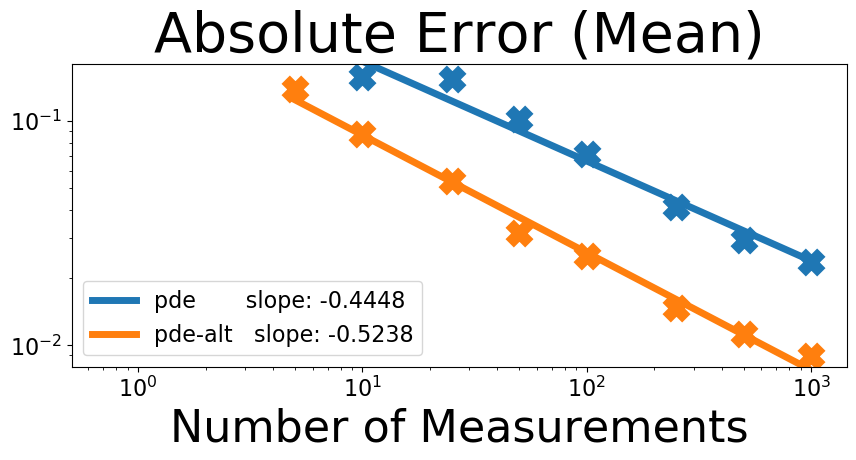
\includegraphics[width=0.475\linewidth]{figures/pde/pde_convergence_mud_obs_mean}
  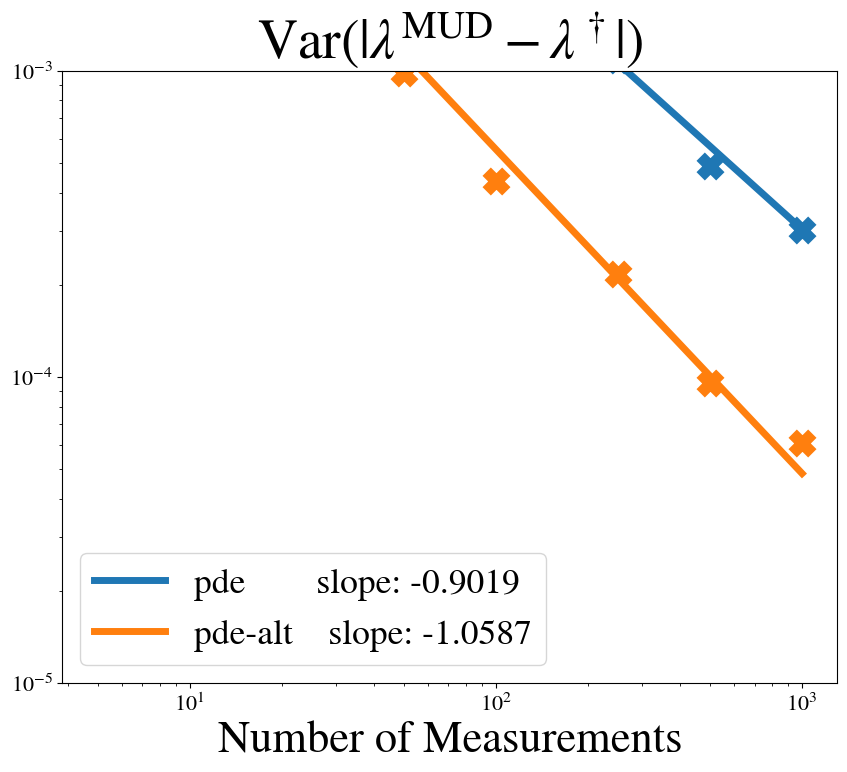
\includegraphics[width=0.475\linewidth]{figures/pde/pde_convergence_mud_obs_var}
  \caption{Convergence of the MUD point (given $N=1E4$ model evaluations) for increasing numbers of observations for randomly placed sensors.
  We observe similar rates of convergence for both arrangements of measurement locations, with a marked improvement in both accuracy and precision when an informed placement is used.
  }
  \label{fig:pde-convergence-obs}
\end{figure}


Similar to \ref{fig:ode-convergence-std}, we demonstrate that using more sensitive measurement equipment improves the estimation of the MUD point.
Again we consider choices of standard deviation associated with $\tau = 0.1, 0.05, 0.01, 0.005, \text{ and } 0.001$ for $\mathbb{P}( \abs{\xi} < \tau ) = 99\%$
In Figure~\ref{fig:pde-convergence-std}, we study the impact of more precise measurement equipment on the absolute error's mean and variance.

\begin{figure}[htbp]
  \centering
  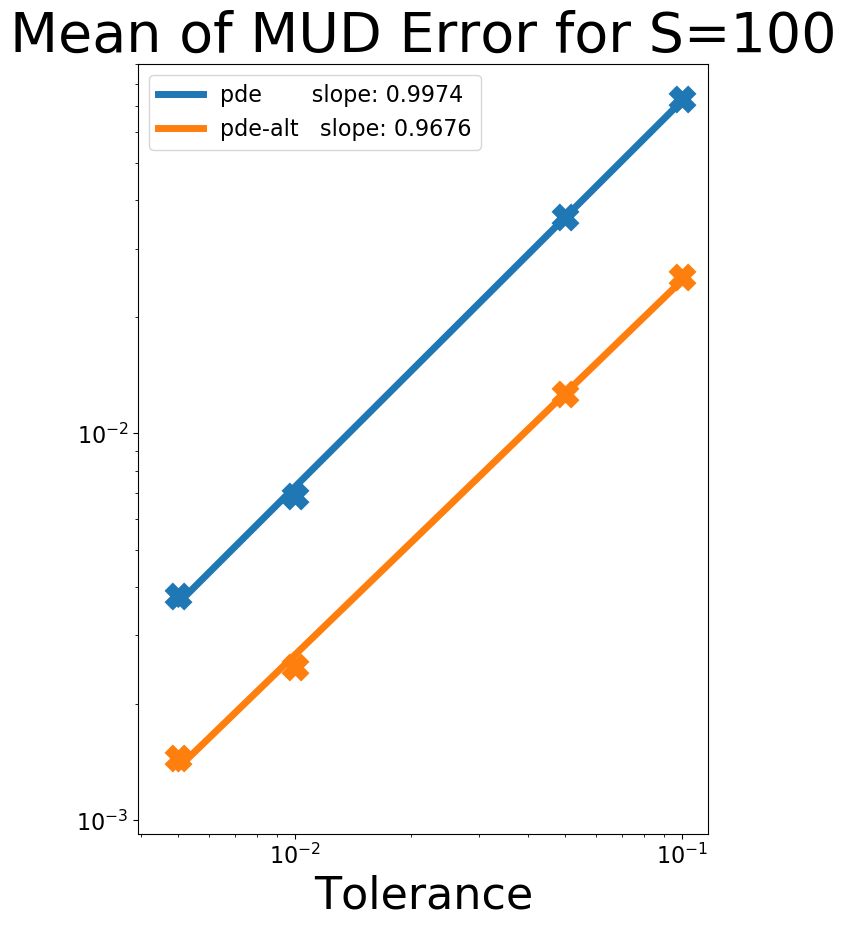
\includegraphics[width=0.475\linewidth]{figures/pde/pde_convergence_mud_std_mean}
  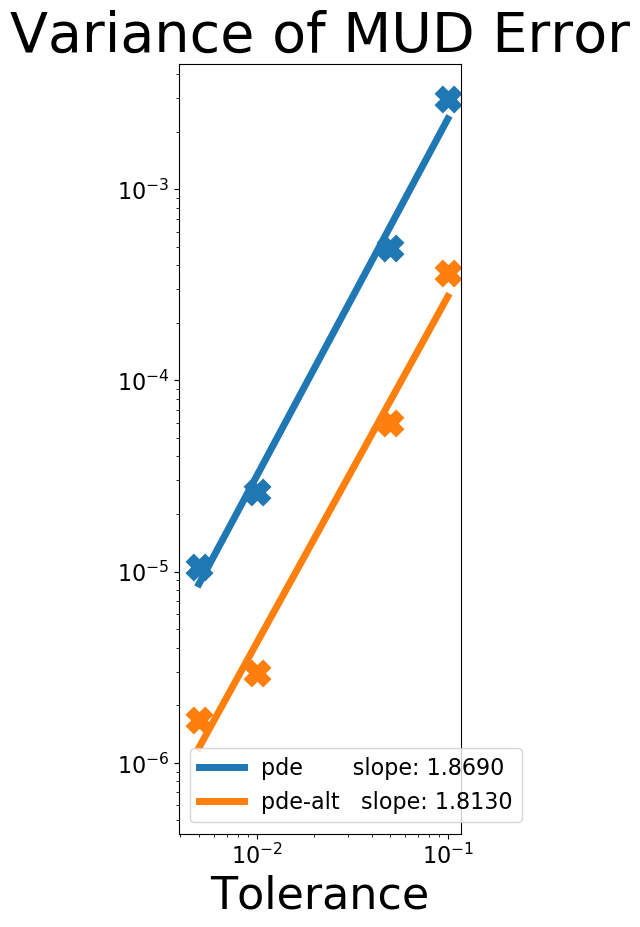
\includegraphics[width=0.475\linewidth]{figures/pde/pde_convergence_mud_std_var}
  \caption{Convergence of the MUD point given $N=1E4$ model evaluations for different measurement precisions for randomly placed sensors, incorporating $S=100$ measurements.
  We note that the convergence rates are the same but the overall accuracy and precision improve when sensors are placed in regions of $u$ that exhibit higher sensitivity to changes in $\param$.
  }
  \label{fig:pde-convergence-std}
\end{figure}


These results demonstrate that even randomly placed sensors in the interior of $\Omega$ are suitable for parameter estimation.
Figure~\ref{fig:pde-ref-solution} shows the twenty most sensitive sensors appear by the left boundary of the domain; choosing sensors more carefully using this information could lead to improved accuracy with fewer sensors.
Let us turn our attention to incroporating this observation into our experimental design chocies.

\subsubsection{Informed Sensor Placement}
Instead of placing sensors throughout the square interior of $\Omega$ given by $(0.05, 0.95)^2$, we briefly consider how the convergence results would change if the subdomain for sensors was better chosen to be near the left boundary.
Furthermore, the response surface exhibits horizontal symmetry, so we restrict locations to the bottom half of $\Omega$.
We perform the same experiment for sensors placed in $(0.05, 0.25)\times(0.05, 0.5)$ and show the results in

We demonstrate the sensitivities of each sensor in the right half of Figure~\ref{fig:pde-sensitivity}, and note that there are fewer sensors twhich exhibit low sensitivity to changes in $\param$.
It appears in the right half of Figure~\ref{fig:pde-convergence-obs}, that two decimal places of accuracy can be achieved with approximately $250$ samples instead of the $1000$ required in the left-half.


TK - Closing statements about optimal experimental design being out of the scope of this work, but how this was an interesting thing to observe.

%%%%%%%%%%%%%%%%%%%%%%%%%%%%%%%%%%%%%%%%%%%%%%%%%%%%%%%%%%%%%%%%%%%%
%%%%%%%%%%%%%%%%%%%%%%%%%%%%%%%%%%%%%%%%%%%%%%%%%%%%%%%%%%%%%%%%%%%%

%%%%%%%%%%%%%%%%%%%%%%%%%%%%%%%%%%%%%%%%%%%%%%%%%%%%%%%%%%%%%%%%%%%%
%%%%%%%%%%%%%%%%%%%%%%%%%%%%%%%%%%%%%%%%%%%%%%%%%%%%%%%%%%%%%%%%%%%%
\subsection{Concluding Remarks for Examples}

As these examples demonstrate, Data--Consistent Inversion can be used for parameter identification as a viable alternative to existing methods.
These problems have involved one-dimensional input and output spaces, and so the resulting problems were not necessarily ones that would benefit from regularization.

We point out that in the framework of collapsing available observations of data leaves the output space as scalar-valued.
As the number of parameters grows, this output dimension effectively stays fixed.
This is particularly when the DCI approach becomes advantageous.
One can incorporate a much wider variety of prior beliefs about the relative likelihoods of parameters before data is collected without compromising predictive error.
The DCI approach guarantees that the functional defined (for us, the weighted mean error) will remain accurate in spite of any encoded assumptions that are somehow at odds with data that is subsequently collected.

%%%%%%%%%%%%%%%%%%%%%%%%%%%%%%%%%%%%%%%%%%%%%%%%%%%%%%%%%%%%%%%%%%%%
%%%%%%%%%%%%%%%%%%%%%%%%%%%%%%%%%%%%%%%%%%%%%%%%%%%%%%%%%%%%%%%%%%%%

\FloatBarrier

\section{Extension to Vector-Valued QoI Maps}
The examples in Sections~\ref{subsec:ode-example} and \ref{subsec:pde-example} motivate the use of a data-constructed QoI in order to incorporate an arbitrary number of measurements in a system into a scalar-valued map.
These examples were chosen so that $\text{dim}({\Lambda}) = 1$ for simplicity and to establish a baseline for convergence results.
The linear examples in Section~\ref{subsec:high-dim-linear-example} demonstrate that the DCI framework maintains the accuracy of least-squares while incorporating initial beliefs for higher-dimensional linear maps.
In those examples, we showed that our ability to resolve a true parameter improved as the gap between input dimension and operator row-rank shrunk.

The rank-deficiency of an operator can be attributed either to ill-conditioning of an operator $A:P\to P$, or when $P>D$ for a full-rank $A:P\to D$.
In scenarios where $S>P$ observations are available, we are motivated to somehow leverage the form of Eq.~\eqref{eq:qoi_WME} to construct a vector-valued version incorporating subsets of $S$ for each component.
For example, a system for which spatial measurements are available over time may motivate constructing a scalar-valued WME map for each spatial location.
If distinctly different observable quantities are available (ones perhaps with different physical units), then these may be collapsed into each component of the map.

The discussion of how to optimally construct such maps is beyond the scope of this work, and would need to take into account nuances involving measurement sensitivities and address combinatorial design-spaces.
However, we summarize that the extension of the equations presented in Section~\ref{sec:MUD_analysis} follows directly by constructing the resultant $1\times P$ matrices $A$ and scalar-valued $b$ for each component and then stacking them to form a $D\times P$ system, where we are motivated to minimize $P-D$.

%%%%%%%%%%%%%%%%%%%%%%%%%%%%%%%%%%%%%%%%%%%%%%%%%%%%%%%%%%%%%%%%%%%%
%%%%%%%%%%%%%%%%%%%%%%%%%%%%%%%%%%%%%%%%%%%%%%%%%%%%%%%%%%%%%%%%%%%%

\subsection{A Vector-Valued QoI Map}
In the previous example, we presumed a fair bit of prior knowledge about the structure of $g$ being a sine curve; we only had to estimate a scaling coefficient for it.
To demonstrate the use of the WME QoI in solving inverse problems in higher dimensions, we set up the following series of examples in the same spirit as the former, presuming less about $g$ than before.
Suppose we know that $g$ is negative and bounded below by $-4$, and we pursue estimating it by first placing two knots on the interior of the domain of $g$ and estimating its value at these points.
This gives us a parameter space of $\pspace = [-4, 0]$, and we choose a polynomial function $g$ which exhibits similar behavior to the former $\sin$ curve, but without the symmetry about $x_2=0.5$, and scale it so that it takes a minimum at the same value as before (at $-3$).
Over this space we will assume a uniform density again.
We selected $g(x) = \alpha x_2^2 (x_2 - 1)^5$, with $\alpha$ chosen to satisfy the aforementioned design specification (so that $g(x)=-3$ for $x=(0,\frac{2}{7})$).

Our first two knots will be the equispaced points $x = (0,\frac{1}{3}), (0,\frac{2}{3})$, and the family of functions that this spans is visually illustrated in the left half of Figure~\ref{fig:pde-highd-initial}, alongside the true function and the associated piecewise--linear that comes from interpolating the true $g$.
The rest of the problem setup will be kept the same as the previous example, except that instead of $N=10,000$ parameter space samples, we use $1,000$.
The reason for this is that we will not be doing the same convergence studies, so we are less interested in exhaustively exploring $\pspace$ than demonstrating that our method can handle a wider variety of inverse problems than the previous examples may suggest.


\begin{figure}
\centering
  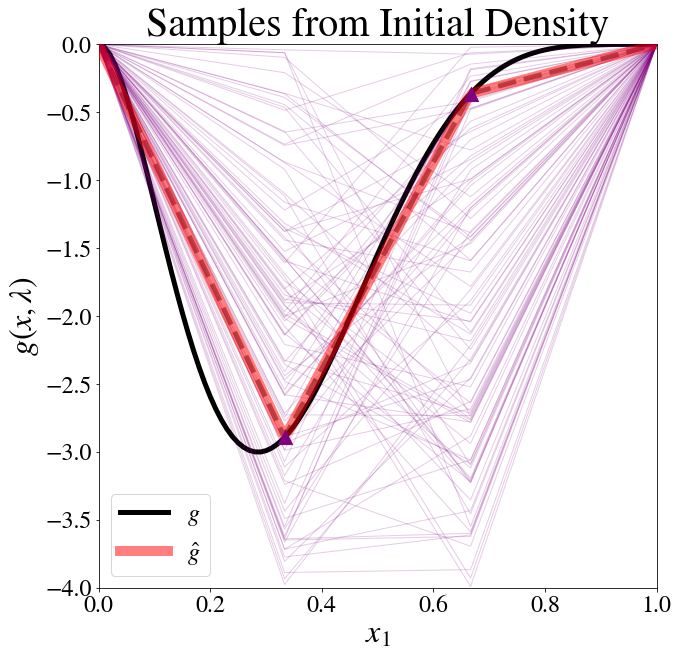
\includegraphics[width=0.475\linewidth]{figures/pde-highd/pde-highd_init_D2.png}
  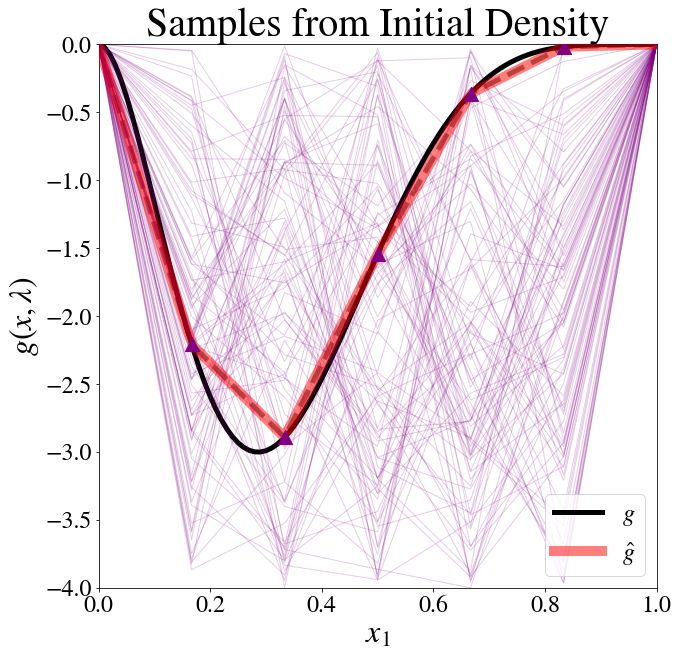
\includegraphics[width=0.475\linewidth]{figures/pde-highd/pde-highd_init_D5.png}
\caption{
One thousand initial parameter samples (our model evaluation ``bugdet'') were used to estimate $g$, constructed by taking independent uniform samples from $[-4, 0]$ for each direction are shown in gray. (Left): Two-knot problem. (Right): Five-knot problem.
}
\label{fig:pde-highd-initial}
\end{figure}

\subsubsection{A Scalar-Valued QoI Map}

Our first inverse problem will involve solving the SIP with the same scalar-valued QoI map constructed by incorporating all the measurements into \eqref{eq:qoi_WME}, and to give the reader a sense of the ability for this ``basis'' to match the one-hundred measurements used for inversion, we plot the best match of our thousand parameter samples with respect to these measurements in purple in the top half of Figure~\ref{fig:pde-highd-2d-scalar-mud}.
There, we also plot the closest match to the interpolating piecewise-linear function in green, and note that we have a near-identical match among our thousand parameter samples, though the best predictor of the data we collected is a different sample.
We are curious which of these two functions the MUD will more closely resemble.
The residual Q-Q plots for the two functions are shown to illustrate the differences in misfit to provide an alternative view to the goodness-of-fit.


\begin{figure}
\centering
  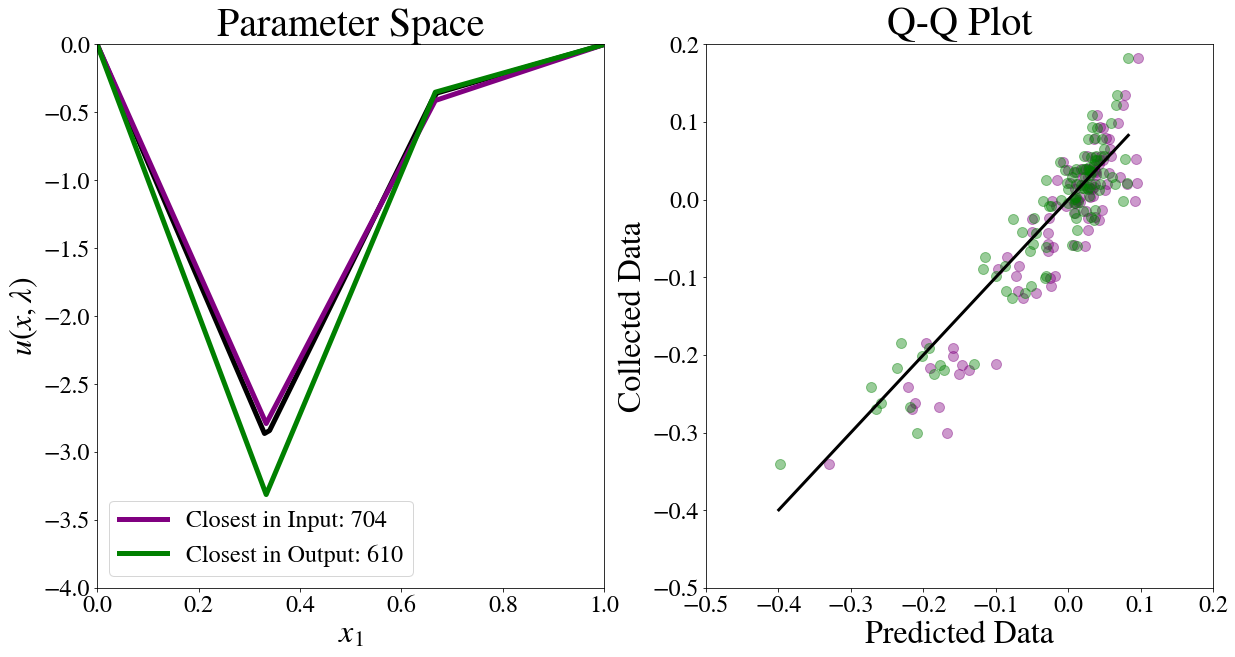
\includegraphics[width=0.95\linewidth]{figures/pde-highd/pde-highd_proj_D2.png}
  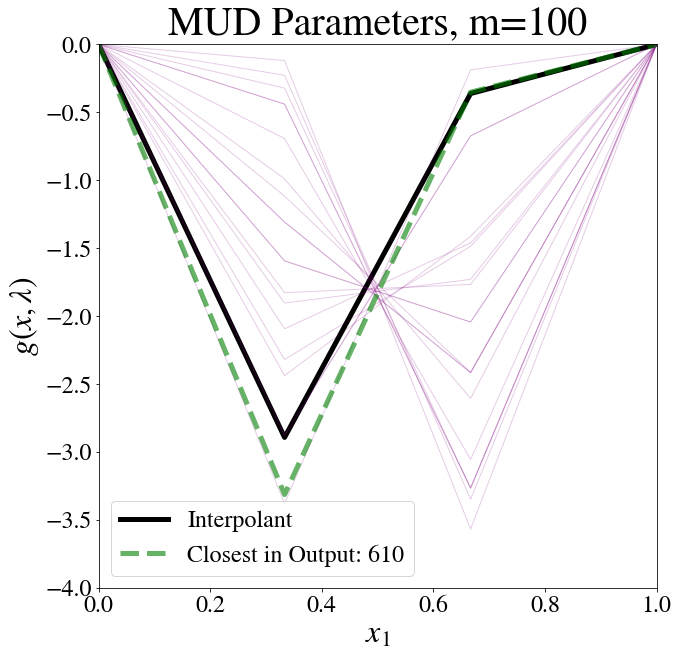
\includegraphics[width=0.95\linewidth]{figures/pde-highd/pde-highd_pair_D2-1_m100.png}
\caption{
}
\label{fig:pde-highd-2d-scalar-mud}
\end{figure}

In the bottom half of \ref{fig:pde-highd-2d-scalar-mud}, we show the MUD solutions arising from twenty trials using different observations of noise.
Of particular interest is that the solutions seem to discover one of two types of explanations for the data, seemingly unable to decide which half of the domain represents a better estimate of $g$'s minimum value.
As mentioned, this set of solutions comes from collapsing all hundred measurements into a scalar--valued QoI map, which negatively impacts our ability to identify the parameter in the problem, since our SIP is now $2\rightarrow 1$.
[TK - cite Troy's result about dimensions from AWR paper] implies that we have an incentive to construct maps which ``close the gap'', so to speak, between input and output dimension, to fully leverage the geometry of available information.
This can be seen in the contour structure of the updated density samples plotted in red in \ref{fig:pde-highd-2d-example}.


\FloatBarrier
\subsubsection{Some (Options for) Vector-Valued QoI Maps}

Suppose that instead of constructing a scalar--valued QoI map, we used the form of \eqref{eq:qoi_WME} to construct a map with two components, yielding a $2 \rightarrow 2$ SIP instead.
Would such an approach provide any tangible benefit for resolving the uncertainty in our true function $g$?
To explore this question, we propose two relatively uninteresting methods for splitting our hundred measurements in to two sets which will be used to construct each component of the map according to \eqref{eq:qoi_WME}.
Both are shown in the top half of Figure~\ref{fig:pde-highd-2d-geometry}, and represent a bisection through $\Omega$ vertically and horizontally.

\begin{figure}
\centering
  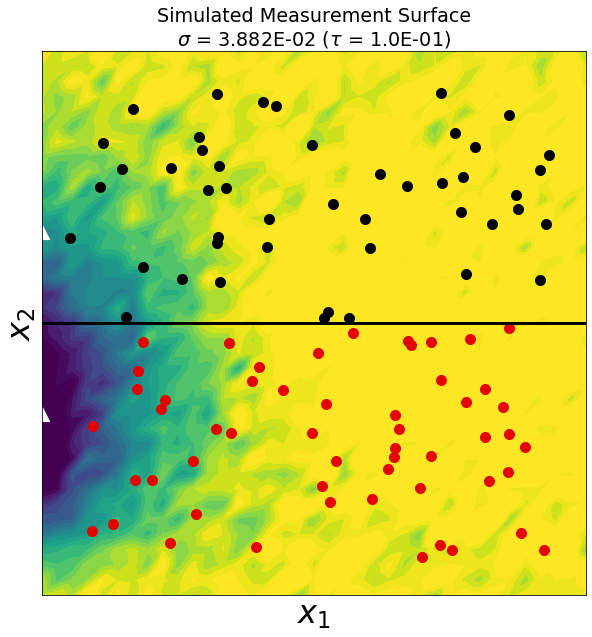
\includegraphics[width=0.475\linewidth]{figures/pde-highd/pde-highd_sensors_D2.png}
  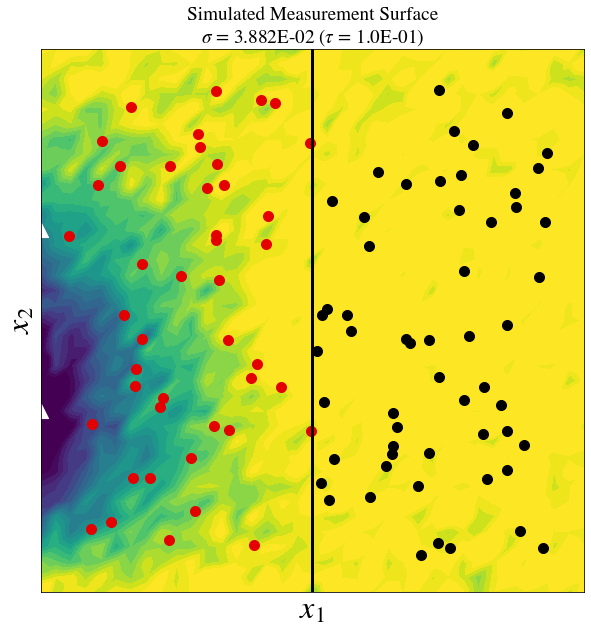
\includegraphics[width=0.475\linewidth]{figures/pde-highd/pde-highd_sensors-alt_D2.png}
  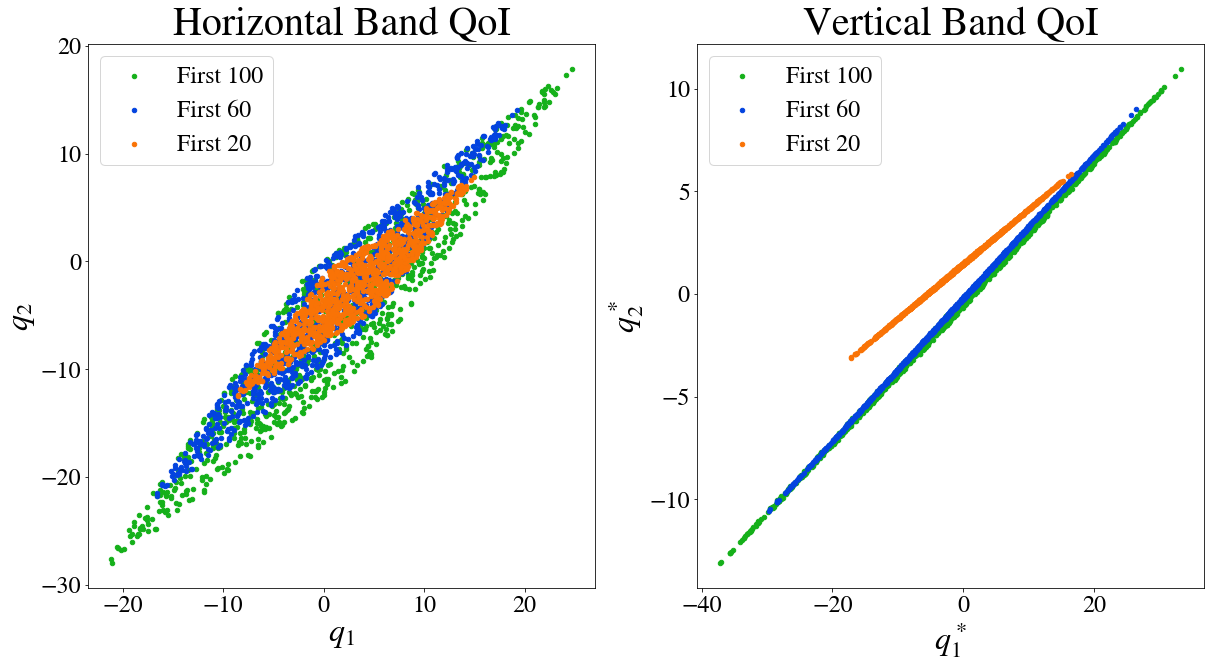
\includegraphics[width=0.95\linewidth]{figures/pde-highd/pde-highd_geom_D2.png}
\caption{
(Bottom): The vector-valued QoI map is constructed for all $N=10,000$ parameter evaluations and the two resulting vectors are plotted against one another for both methods of partitioning $\Omega$.
}
\label{fig:pde-highd-2d-geometry}
\end{figure}

There are now two QoI maps under consideration, which should we use?
Before solving an inverse problem, there are a-priori analysis that can be performed that can provide heuristics to help address these questions.
We first evaluate our thousand parameter samples through each of these maps and inspect the two-dimensional scatter-plots to build intuition about the underlying geometry induced by these maps.
We repeat this process for three subsets of the measurements (using the first samples in each half of $\Omega$ according to the random index assigned to them), and demonstrate the two resulting sets of relationship in the bottom half of Figure~\ref{fig:pde-highd-2d-geometry}.
This figure also shows the associated designs against the noisy response surface as a backdrop.

\subsubsection{An Aside for Geometric Considerations}

First, we note that the inclusion of more data points has the effect of dilating (and to some extent rotating) the induced data space for both QoI maps.
The geometric implication of this in the context of the chosen form of the QoI map has an interesting consequence.
Recall that the observed distribution remains a standard Gaussian, regardless of the number of data points used to construct the map.
In two dimensions, this observed distribution becomes a multivariate normal distribution instead, which can be visually thought of as a circular ``target'' located in the middle of each of the scatter-plots in Fig. \ref{fig:pde-highd-2d-geometry}.
As more measurements are incorporated, the size of that target relative to the rest of the space becomes increasingly small since the data manifolds dilate.
If the reader would indulge the author in another metaphor, it is akin to finding the same needle in larger piles of hay.
More is asked of the solution to the SIP, since there are more measurements with which the model must agree.

The second implication of the two ways in which the maps can be formed is more visually evident, as the two quantities of interest that arise from a vertical bisection of $\Omega$ are nearly perfectly correlated.
The two maps are presenting almost the same information (the shapes are very slim parallelograms), and so we fundamentally can already expect there to be very little difference between MUD points arising from using this map when compared to using the scalar--valued map.
Particularly since the observed distribution is radially symmetric, this problem\---while technically two-dimensional\---appears to be one-dimensional.

By contrast, the map induced by a horizontal split (bottom left of Fig. \ref{fig:pde-highd-2d-geometry}) provides new information in each component.
While there is some correlation (the manifolds are not rectangular), a far greater proportion of samples will fall within the practical support of the observed distribution, which qualifies them as possible solutions to the SIP.
More information is learned with the inclusion of each component using this design than would be with the vertical split.

To this end, for the sake of brevity, we focus our attention on comparing the horizontal vector--valued QoI map to the scalar one, and note that a more fulfilling discussion of constructing QoI maps that induce desirable geometric properties is of interest for future work.
For the remainder of this example, the ``vector--valued'' map will refer to the the one which is split horizontally, and we note that this design, while not having any guarantees of optimality for precision or accuracy's sake, at least respects the flow of information in the system being studied.
Since $\param$ is parameterizing the left Neumann boundary condition, information about its state flows from left to right in the horizontal direction.



\FloatBarrier
\subsubsection{Comparing Solutions}

We turn the reader's attention to Figure~\ref{fig:pde-highd-2d-example}, which illustrates an example MUD solution for both the scalar-- and vector--valued QoI maps.
The predicted response surfaces are shown at the top, and the associated functions and residual plots are below it.
In this particular instance, it appears that the vector-valued MUD solution does a better job capturing the qualitative behavior of $g$; the difference in the residuals is less pronounced.
Both solutions manage to capture some general behavior of the true function, but to better understand the differences in the two solutions, we need instead to look at the set of probable samples, not only the most likely among them.

\begin{figure}[htbp]
\centering
  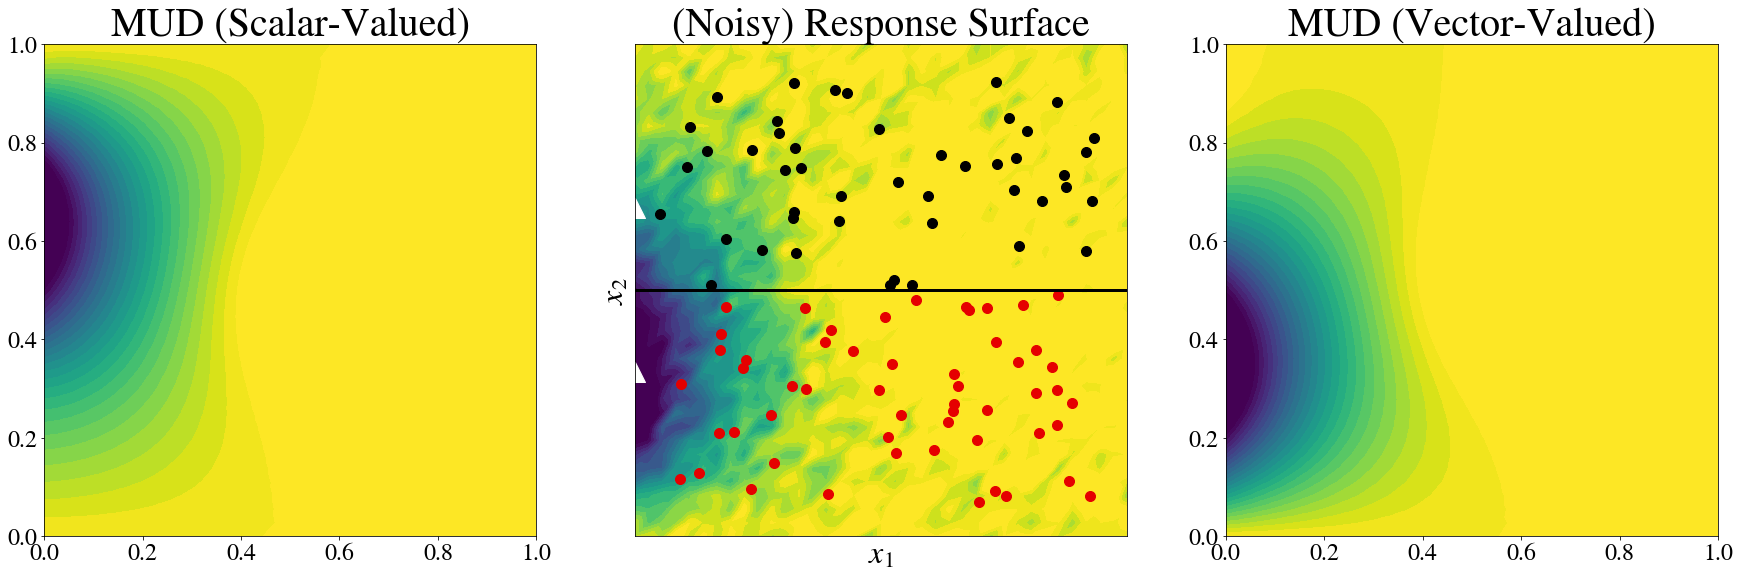
\includegraphics[width=0.95\linewidth]{figures/pde-highd/pde-highd_surf_exmud_D2_m100.png}
  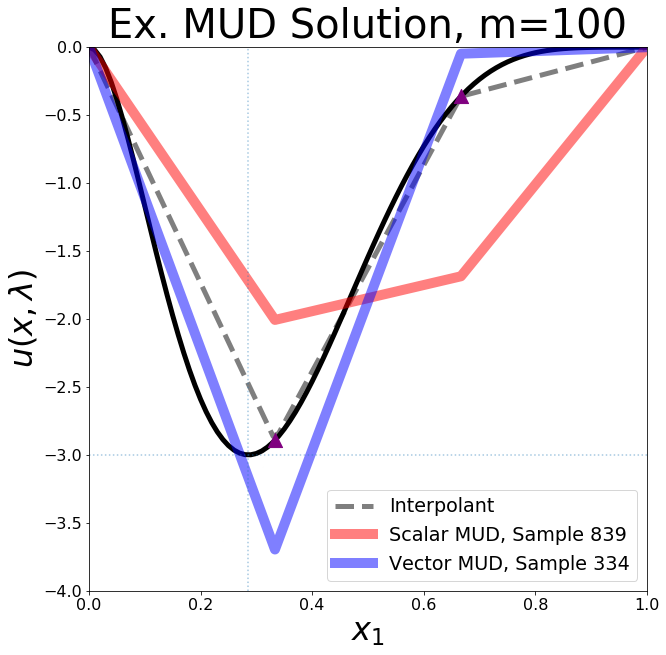
\includegraphics[width=0.6\linewidth]{figures/pde-highd/pde-highd_comp_exmud_D2_m100.png}
\caption{
100 measurements
}
\label{fig:pde-highd-2d-example}
\end{figure}


This is what is shown at the bottom of Fig.~\ref{fig:pde-highd-2d-scatter}: we normalize our ratio pdf evaluations and plot the samples that exceed two thresholds, numerical zero (left), and $1/N$ (right) to give some sense of samples that may come from accept/reject algorithms (since our initial was uniform).
Both scatter-plots exhibit the same geometry, appearing to trace a band through the parameter space.
Fundamentally, at first glance at the left figure, it is already apparent that half of $\Lambda$ has been ruled out, and that the correlation structure between the two knots has been discovered.
The vector--valued samples, however, cluster more tightly around the optimal samples (the ``projection'' here refers to the sample which minimizes the 2-norm to the noiseless data).
The incorporation of two directions instead of one whittles away more of the parameter space as being less relatively likely.
If we were to perform accept/reject, the resulting set would be fairly well constrained to the upper-lefthand corner of the two-dimensional parameter space.

\begin{figure}[htbp]
\centering
  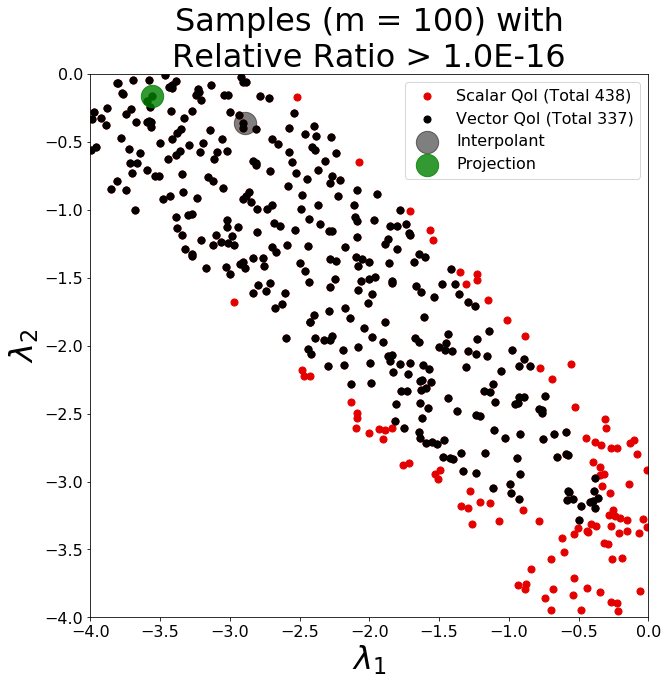
\includegraphics[width=0.45\linewidth]{figures/pde-highd/pde-highd_update_scatter_D2_t1-0E-16.png}
  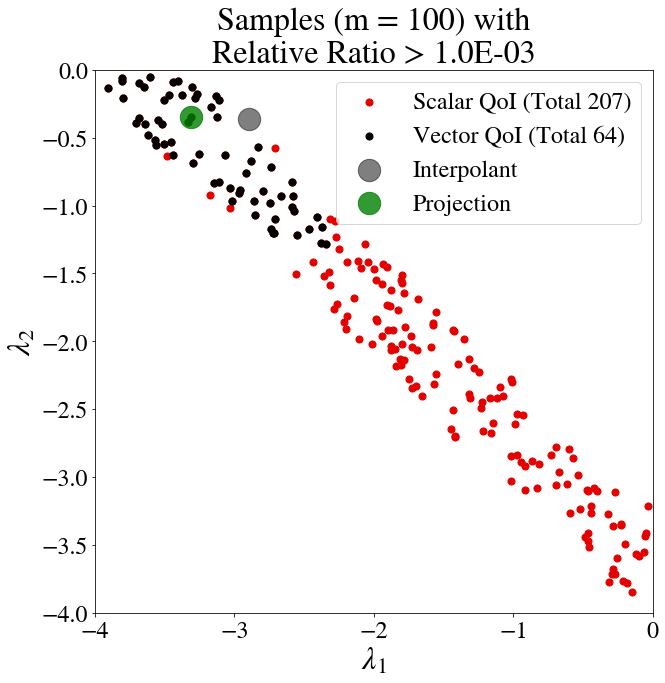
\includegraphics[width=0.45\linewidth]{figures/pde-highd/pde-highd_update_scatter_D2_t1-0E-03.png}
\caption{
100 measurements
}
\label{fig:pde-highd-2d-scatter}
\end{figure}

To rule out the possibility that our one updated density / MUD point was luck, we again re-solve our SIP for twenty different realizations of noise to pollute our hundred measurements, and show the resulting solutions for the first twenty and all hundred being used to construct the vector--valued map.
The resulting functions that are induced by these MUD points are shown in Fig.~\ref{fig:pde-highd-2d-vector-mud}, and we note that solutions are no longer are considering the possibility of the minimum value of $g$ being at the wrong knot point as we saw in Fig.~\ref{fig:pde-highd-2d-scalar-mud}, even when only twenty total data points are used to construct $Q$.
By the time all hundred measurements are incorporated, the MUD solutions appear to be tracing out curves between the projection function and the interpolant function, a far more accurate set of predictions than those from the scalar--valued map.

\begin{figure}[htbp]
\centering
  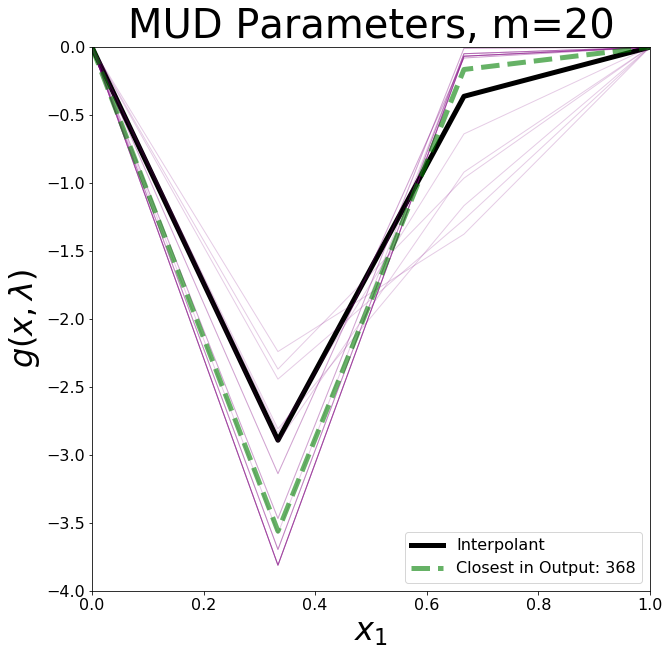
\includegraphics[width=0.6\linewidth]{figures/pde-highd/pde-highd_pair_D2-2_m20.png}
  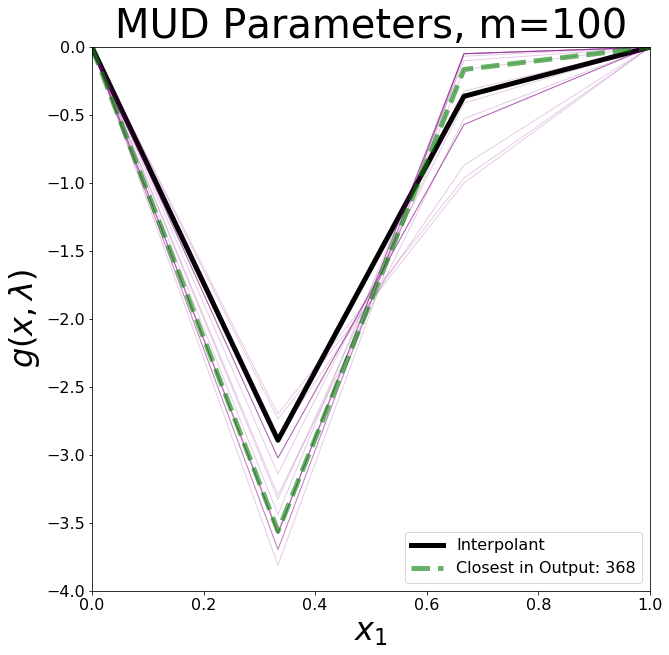
\includegraphics[width=0.6\linewidth]{figures/pde-highd/pde-highd_pair_D2-2_m100.png}
\caption{
(Top): When vectorizing our QoI map, we find that we are able to achieve more accuracy with fewer measurements. Here, we see far less variation in MUD solutions than in the bottom of Fig.~\ref{fig:pde-highd-2d-scalar-mud}.
(Bottom): When all 100 measurements are incorporated
}
\label{fig:pde-highd-2d-vector-mud}
\end{figure}

How we incorporate the available data has a dramatic impact on our ability to reduce uncertainty in the parameter space.
We attempt to illustrate this by requesting the reader juxtapose figures of the initial samples in \ref{fig:pde-highd-initial} to those in \ref{fig:pde-highd-2d-scalar-mud} and \ref{fig:pde-highd-2d-vector-mud}.
To better quantify the differences, it is more rigorous to study how close we are to $g$ (in function space).
Since the approximation $\hat{g}$ that arises from evaluating the MUD point is piecewise-linear, and $g$ is continuous, we use the knot points and the trapezoidal rule to approximate the $L^2$ norm of $\abs{g - \hat{g}}$ (using {\tt scipy}), and plot the resulting histograms for the scalar- and vector-valued $\param$s whose relative ratios exceeded a threshold, and compare them against samples from the initial density, and show the result in Figure~\ref{fig:pde-highd-2d-hist}.


\begin{figure}[htbp]
\centering
  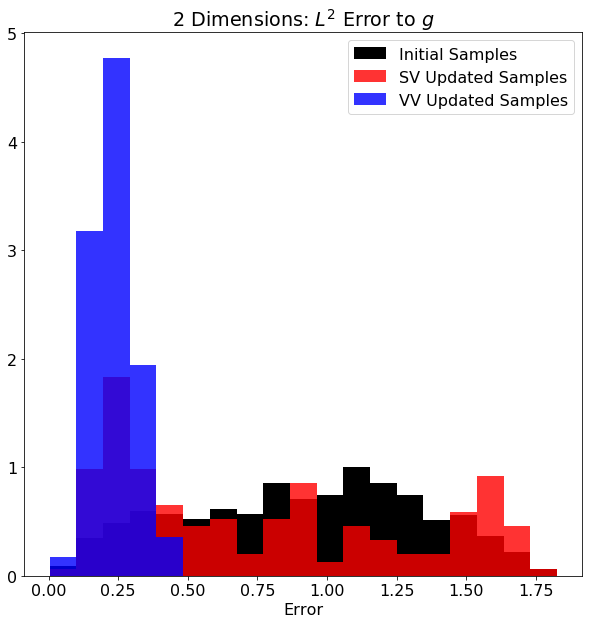
\includegraphics[width=0.675\linewidth]{figures/pde-highd/pde-highd_hist_D2_t5-0E-01}
\caption{
Histograms comparing initial samples with the highest probabilities (relative ratio $> 0.5$).
}
\label{fig:pde-highd-2d-hist}
\end{figure}

In \ref{fig:pde-highd-2d-hist}, the histograms have been normalized for comparison, and while the scalar--valued map still does reduce the uncertainty that we started with in our initial density.
The multi-modal nature of this plot shows a lack of resolution that is not experienced at all by the vector--valued solution.
This multi-modal density of probably samples corresponds to the two types of solutions we saw in Figure~\ref{fig:pde-highd-2d-scalar-mud}.
Both QoI maps solve a stochastic inverse problem, but the latter is more respectful of the geometry of the response surface, and so is able to learn significantly more, and bring us modelers far closer to the true function $g$.


%%%%%%%%%%%%%%%%%%%%%%%%%%%%%%%%%%%%%%%%%%%%%%%%%%%%%%%%%%%%%%%%%%%%
%%%%%%%%%%%%%%%%%%%%%%%%%%%%%%%%%%%%%%%%%%%%%%%%%%%%%%%%%%%%%%%%%%%%
\FloatBarrier
%%%%%%%%%%%%%%%%%%%%%%%%%%%%%%%%%%%%%%%%%%%%%%%%%%%%%%%%%%%%%%%%%%%%
%%%%%%%%%%%%%%%%%%%%%%%%%%%%%%%%%%%%%%%%%%%%%%%%%%%%%%%%%%%%%%%%%%%%
\subsection{Extension to Higher Dimensions}

Suppose now that an eager experimenter decided to start with a five--dimensional problem (five knots instead of two), trying to accomplish greater granularity in the ability to estimate $g$, and imposes the same type of uniform initial in each direction, yielding a parameter space of $\Lambda = [-4, 1]^5$.
In Figure~\ref{fig:pde-highd-initial}, we show what such initial functions would look like, and note that many of them appear to exhibit fluctuating behavior for which the mesh ($36\times36$) being used to solve the problem, would not be fine enough to resolve.
In many senses, this choice of initial density induces a lot of noise into the SIP we are hoping to solve, since ``common sense'' from a modeler's perspective may be able to rule out zig-zag functions from wasting model-evaluation budget, which we retain at the same $N=1000$ samples as in the previous 2-D problem.
To get a sense of what the best possible representations in this peculiar choice of ``basis'' could be, we again find the closest match to the interpolant and to the data and plot them alongside residuals in Figure~\ref{fig:pde-5d-proj}.

\begin{figure}[htbp]
\centering
  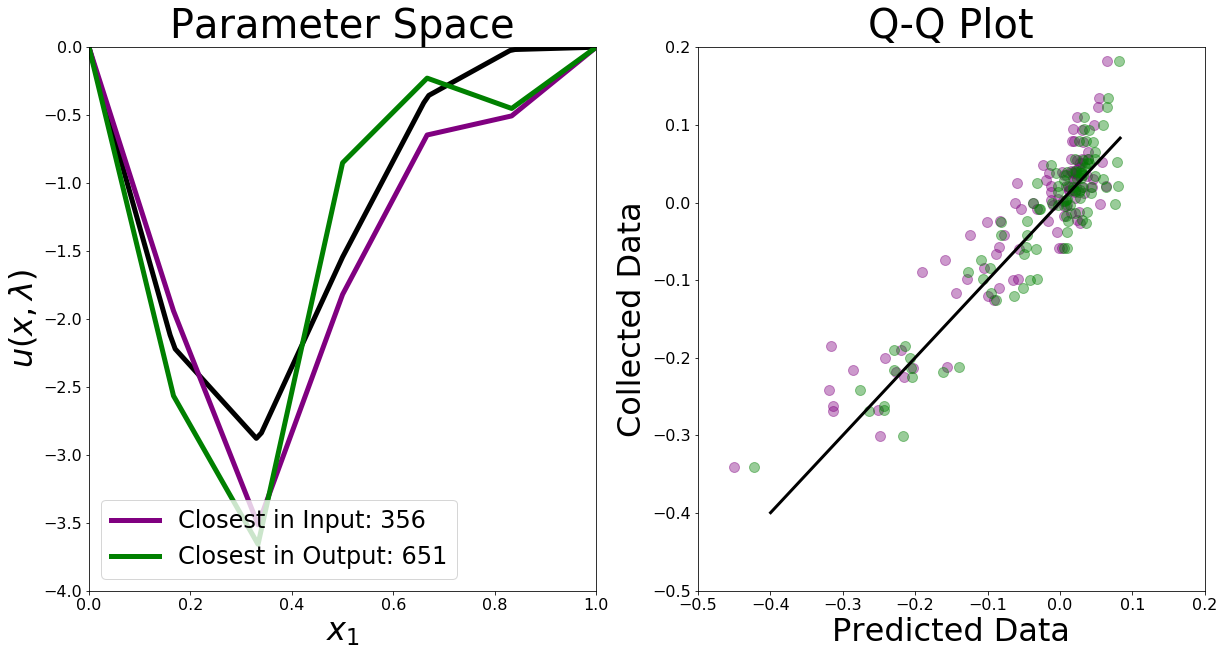
\includegraphics[width=0.675\linewidth]{figures/pde-highd/pde-highd_proj_D5}
\caption{
}
\label{fig:pde-5d-proj}
\end{figure}

Observe that in Figure~\ref{fig:pde-5d-proj}, both the closest fit in parameter and measurement space fail to resolve the true function behavior at $\lambda_5$ (the interpolating piecewise--linear is shown for reference), and both place a minimum at $\lambda_2$.
The plot here is in some sense, the best that can be solved for with this design, and is helpful for comparing against our MUD solutions.
Of particular interest here is to note also is that both functions under-estimate $g$ at $\lambda_2$ by a large margin.
Nevertheless, we pursue the solution for demonstration purposes and solve the SIP for both scalar-- and vector--valued QoI maps, the latter constructed with horizontal bands shown in the bottom left of Figure \ref{fig:pde-highd-5d-example}.

\begin{figure}[htbp]
\centering
  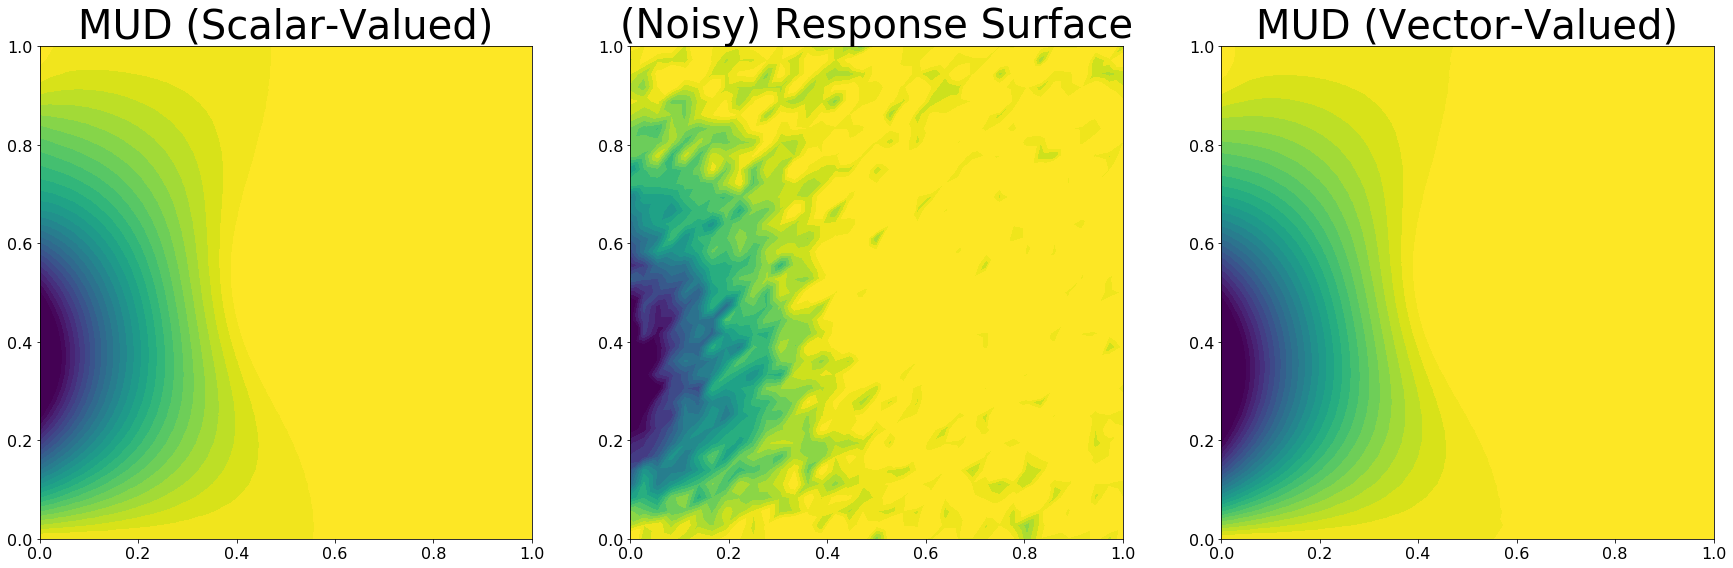
\includegraphics[width=0.95\linewidth]{figures/pde-highd/pde-highd_surf_exmud_D5_m100}
  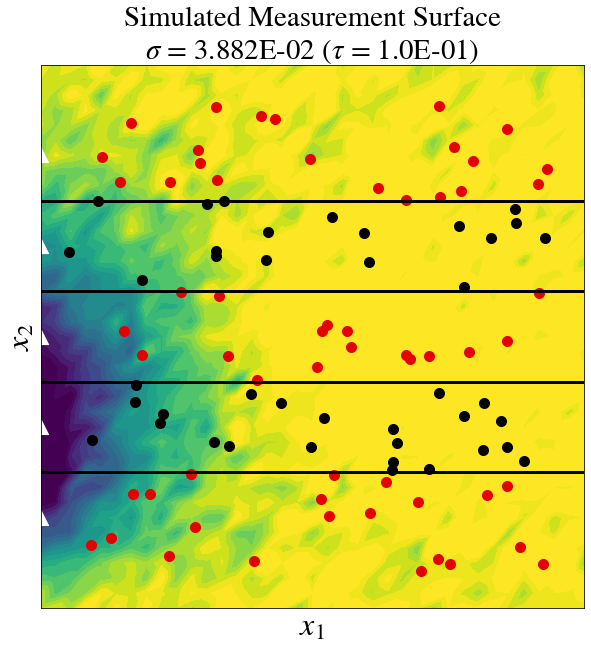
\includegraphics[width=0.35\linewidth]{figures/pde-highd/pde-highd_sensors_D5}
  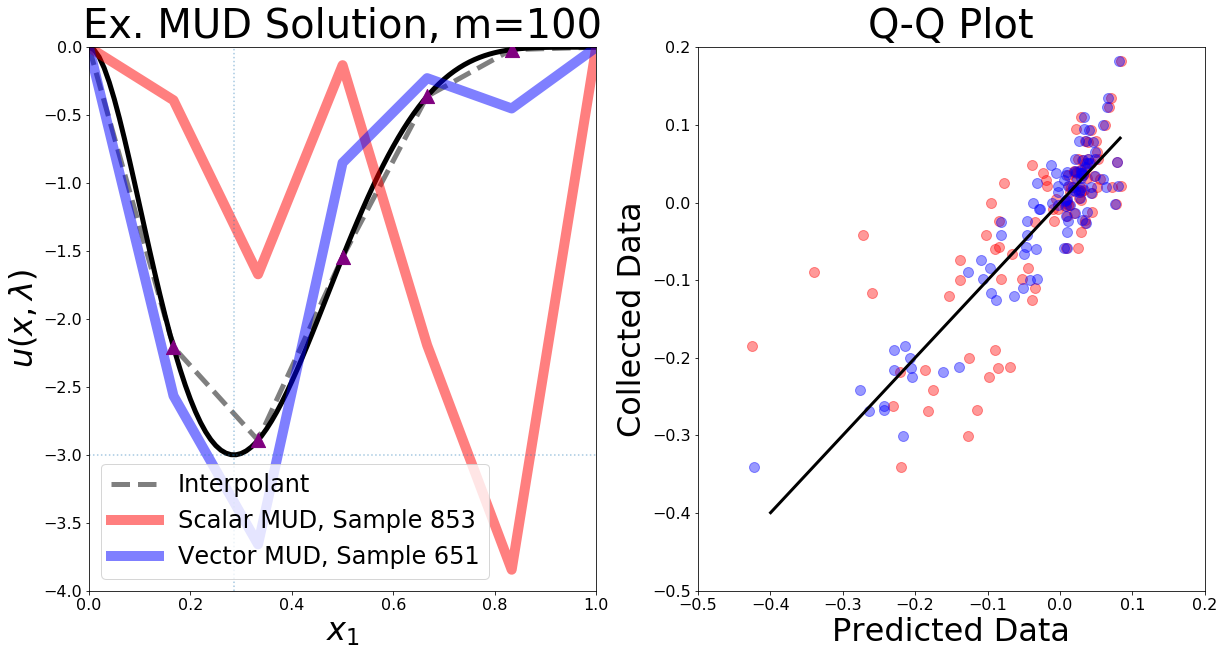
\includegraphics[width=0.6\linewidth]{figures/pde-highd/pde-highd_comp_exmud_D5_m100}
\caption{
(Top): Layout for 5-D vector--valued map and comparison of the two MUD solutions in parameter space.
(Bottom): The response surfaces predicted by the two QoI maps alongside the noisy response surface that generated the simulated collected data.
}
\label{fig:pde-highd-5d-example}
\end{figure}

In Figure~\ref{fig:pde-highd-5d-example}, the scalar-- and vector--valued MUD solutions are shown for the noisy surface plotted in the top-center, with associated predicted response surfaces flanking it.
In the bottom-center plot, we can see that the scalar-valued MUD happens to completely misidentify the location of $g$'s minimum value, but the vector-valued QoI is able to resolve the behavior much better.
In Figure~\ref{fig:pde-highd-5d-mud} we plot the results from twenty repeated trials (perturbations of noise) when using all hundred measurements, and observe the same difference in going from scalar-- to vector--valued solutions for the five--dimensional example that we saw in two dimensions in \ref{fig:pde-highd-2d-scalar-mud}.

\begin{figure}[htbp]
\centering
  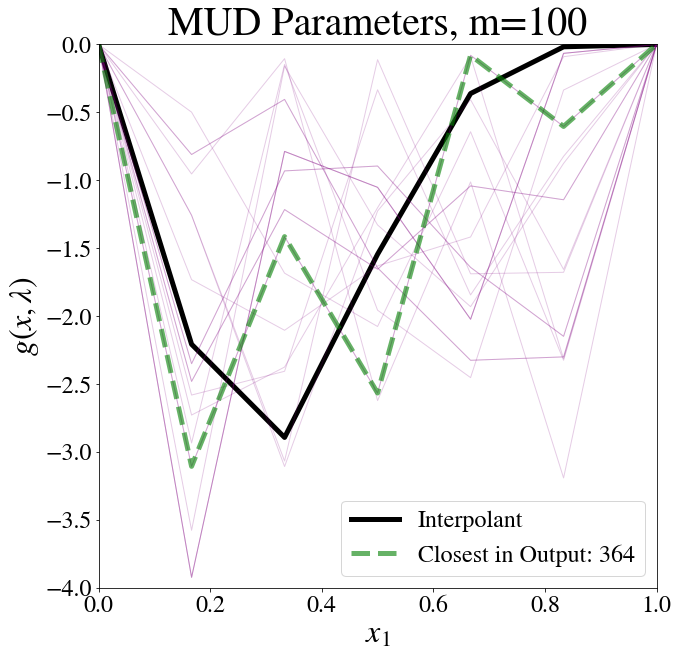
\includegraphics[width=0.95\linewidth]{figures/pde-highd/pde-highd_pair_D5-1_m100}
  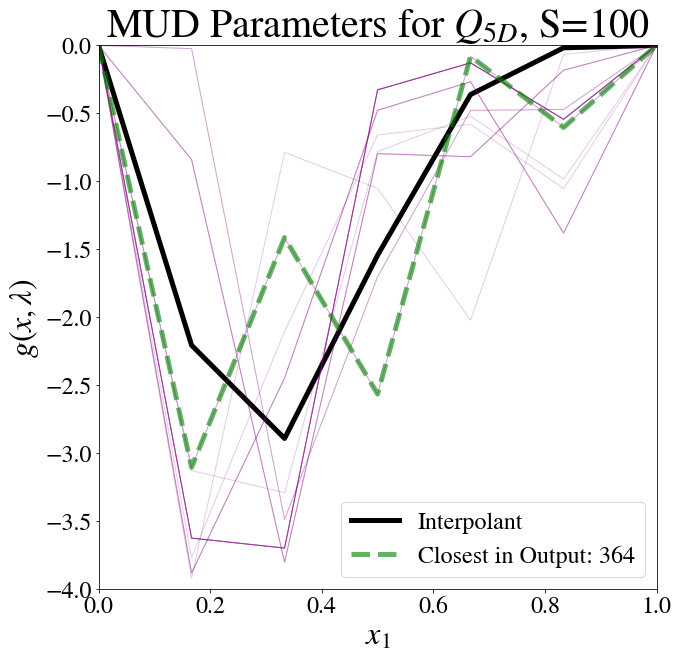
\includegraphics[width=0.95\linewidth]{figures/pde-highd/pde-highd_pair_D5-5_m100}
\caption{
(Top): Scalar-valued solutions.
(Bottom): Vector-valued solutions.
}
\label{fig:pde-highd-5d-mud}
\end{figure}

By increasing the number of quantities of interest used, more directions of uncertainty are resolved in the parameter space.
Since any solution in the equivalence class is a valid one for the SIP, the scalar-valued solutions are much more sensitive to the noise, and so the solutions often appear to identify functions with a minimum on the wrong half of the domain.
In Figure~\ref{fig:pde-highd-5d-mud}, the scalar-valued QoI is unable to differentiate between resolving residual discrepencies in different locations in $\Omega$.
By contrast, the vector-valued QoI is constructed with respect to the flow of information in the system, and so many more of the twenty trials land closer to the true minimum value of $g$.
The solutions for the vector-valued approach instead explore the available knots (at $x_2=1/6$ and $1/3$), nearest the actual minimum value of $2/7$ instead, a much more valuable area of $\Lambda$ to explore.

Perhaps unsurprisingly given the poorly-designed initial density, our MUD solutions still do not really trace out the interpolant that we hope it should in order to approximate $g$.
At the very least, we would hope to accurately estimate the location and value of $g$'s minima.
Recall that we have already solved a two-dimensional version of this problem, which could have been used to inform a much smaller region of two of the five directions to explore.
Let us see what would happen if our initial density was constructed with more care (without needing to use any model evaluations), since we saw from earlier examples that if DCI is initialized at a good initial mean, it has a chance of outperforming even least-squares in resolving discrepency in truth.

%%%%%%%%%%%%%%%%%%%%%%%%%%%%%%%%%%%%%%%%%%%%%%%%%%%%%%%%%%%%%%%%%%%%
%%%%%%%%%%%%%%%%%%%%%%%%%%%%%%%%%%%%%%%%%%%%%%%%%%%%%%%%%%%%%%%%%%%%

\subsection{Alternative Experimental Approach}

[TK - Now we're tying back into the OED discussion]

As we proceed from two to five dimensions, being weary of the fact that we are fighting against the curse of dimensionality, we want to be more intelligent with our specification of an initial density.
Let us take a look at the samples that show up in black on the bottom-right of Figure~\ref{fig:pde-highd-2d-example} from a different perspective.
Instead of looking at high-probability samples as locations in $\Lambda$, let us inspect them as a family of functions that are defined on the unit interval and use the envelope curves they sweep out to inform the specification of a better initial density; consider Figure~\ref{fig:pde-highd-5d-study}.

\begin{figure}[htbp]
\centering
  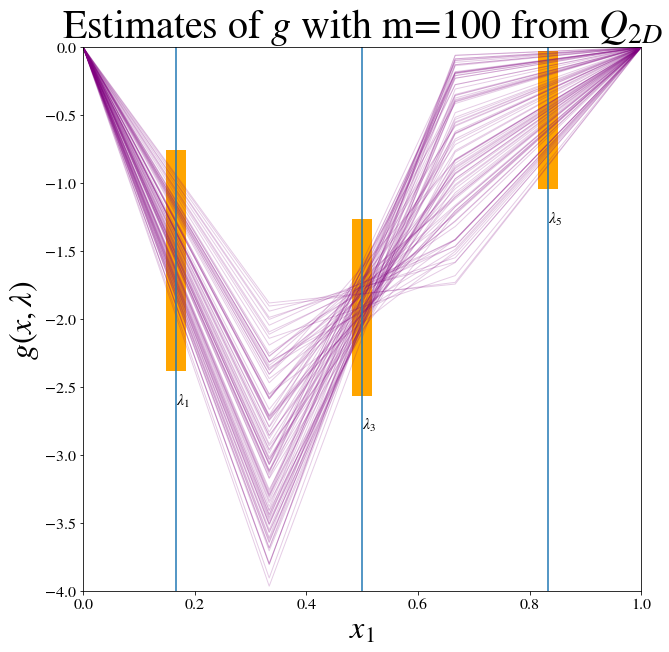
\includegraphics[width=0.675\linewidth]{figures/pde-highd/pde-highd-alt_initial_D5_m100.png}
\caption{
}
\label{fig:pde-highd-5d-study}
\end{figure}

The samples whose relative ratios exceeded $1/1000$ sweep out a family of curves that can be used to estimate bounds not only on $\lambda_2$ and $\lambda_4$ (the previous $\lambda_1$ and $\lambda_2$ from the 2-D problem)\---which exhibit correlation structure that we will turn to momentarily\---but also on the remaining three knots.
To form the intervals shown in orange in Fig.~\ref{fig:pde-highd-5d-study}, we take the upper and lower bounds of the curves passing through the vertical lines drawn at the three new knot values.
To be conservative, we multiply our lower bound by $1.2$ and the upper by $0.8$ (we are still more than halving the interval-length in each direction as compared to the previous 5-D problem).
(Alternatively, one could establish a lower tolerance for accepting likely samples and avoid the multiplication factor, but the authors enjoyed the connection to accepted samples from the updated density).

\subsubsection{A better initial density}
For the two directions remaining, we want to capture the correlation structure that we were able to visually identify in Fig.~\ref{fig:pde-highd-2d-example} and impose something uniform-like on it.
To achieve this, we perform a singular-value decomposition on the likely samples from the \emph{scalar}--valued 2-D solution, since there are so many more samples (it was found to better characterize the direction of the equivalence class, suggesting perhaps a justifiable use for solving the problem with it in such cases).

The singular vectors are used to transform the vector-valued samples, and a uniform sampling is performed over the rectangular bounding box for these points, shown in the center of Figure~\ref{fig:pde-highd-2d-study}.
These generated samples, however, leave $\Lambda$ when transformed back to their native space, as seen in the left panel.
To ameliorate this problem, we instead perform sampling in a while-loop, sampling from this uniform box and rejecting any that would get mapped back outside $\Lambda$.


\begin{figure}[htbp]
\centering
  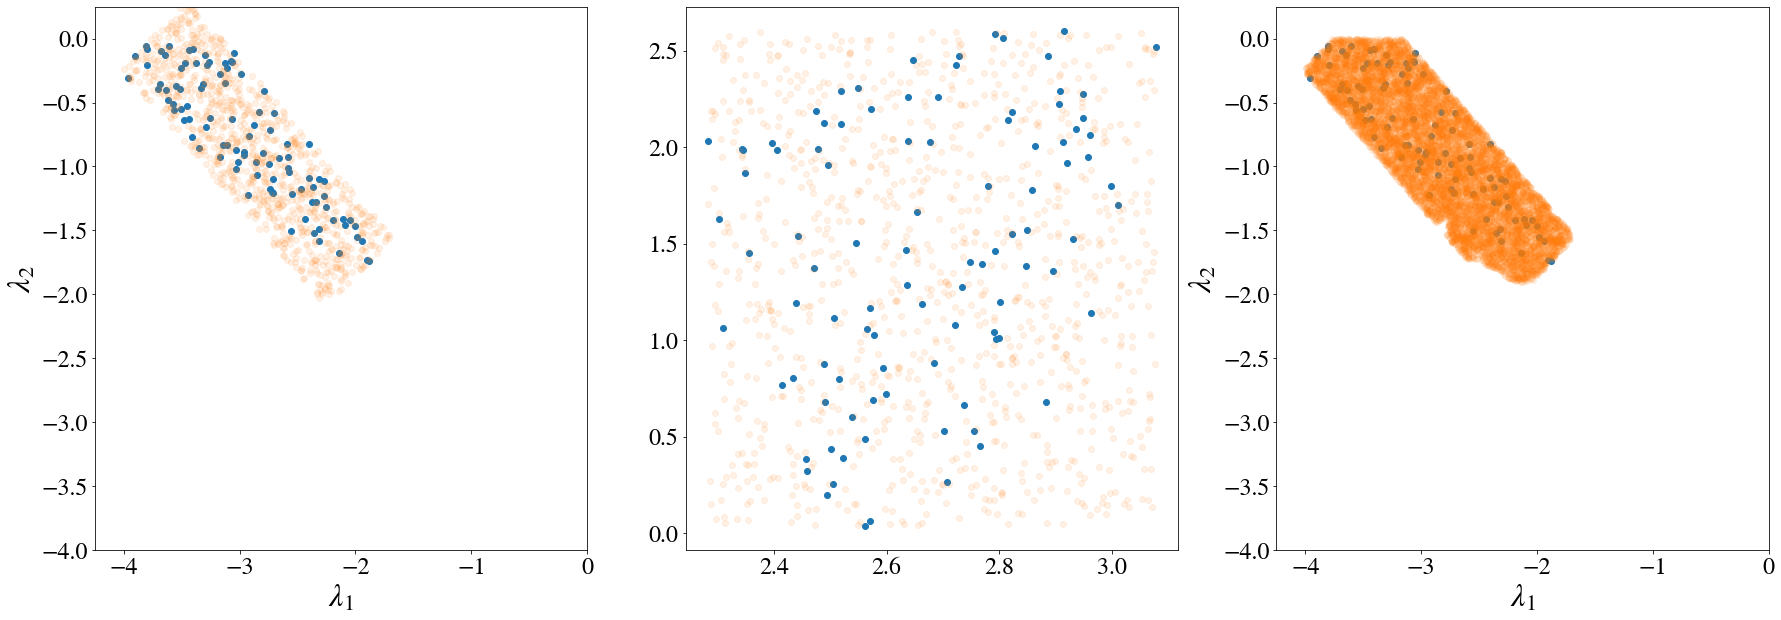
\includegraphics[width=0.95\linewidth]{figures/pde-highd/pde-highd-alt_initial_D2_m100}
\caption{
Generating proposal samples for the two directions informed by solving the 2-D inverse problem, aided by singular-value decompositions and a basic ad-hoc sampling procedure.
}
\label{fig:pde-highd-2d-study}
\end{figure}

Furthermore, note that in the center of the Fig~\ref{fig:pde-highd-2d-study}, there are corner-regions of the space we want to avoid wasting samples on as well, so we reject samples that have squared two-norm greater than $0.05$ from their nearest vector--valued sample.
This sampling procedure produces the set shown in orange on the right side of the figure (ten thousand shown to demonstrate coverage).
In a sense, we wanted to quickly define a computational open cover for the relatively high-probability samples.
We keep one thousand of these 2-D samples, and join them with the three independent uniform sample sets of the same size taken from the intervals in Fig.\ref{fig:pde-highd-5d-study} to form our new initial sample set, the functions from which generate the curves shown in Figure~\ref{fig:pde-highd-5d-init}.

\begin{figure}[htbp]
\centering
  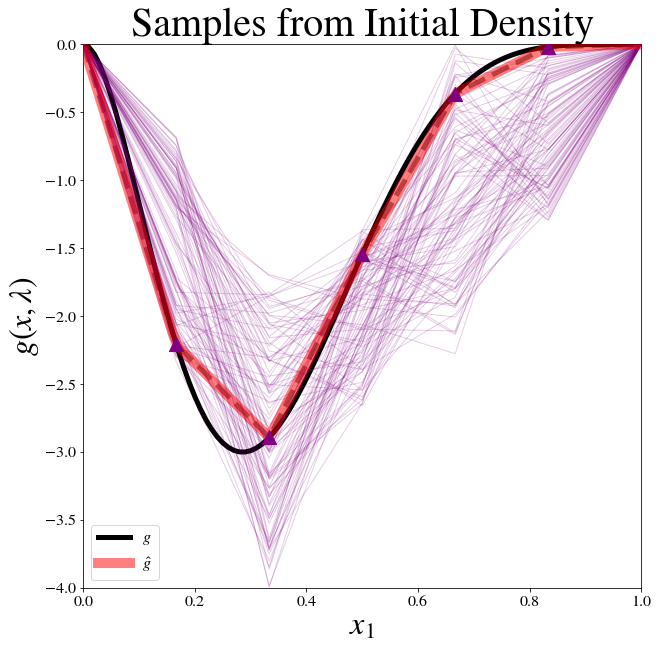
\includegraphics[width=0.675\linewidth]{figures/pde-highd/pde-highd_init_D5-alt}
\caption{
Initial density constructed for the second attempt at the five--dimensional inverse problem, with the structure of solutions learned from the 2-D example incorporated into the selection of bounds in each direction.
}
\label{fig:pde-highd-5d-init}
\end{figure}

These curves, especially when contrasted to those in Fig.~\ref{fig:pde-highd-initial}, represent a far more reasonable set of possibilities, exhibiting none of the erratic roughness that was seen in the first attempt at a five--dimensional initial density.
We note that such considerations of smoothness could be avoided by parameterizing $g$ with a basis of some sort, but that problem is beyond the scope of this already lengthy work.
Another possible improvement would be to incorporate the correlation structure that is present in the three other directions, derivable from a similar SVD-based analysis of the interpolation of the 2-D predictions through the new knot locations, but that would require more visual exploration than the authors deem worthwhile to demonstrate the point they are trying to make.

\begin{figure}[htbp]
\centering
  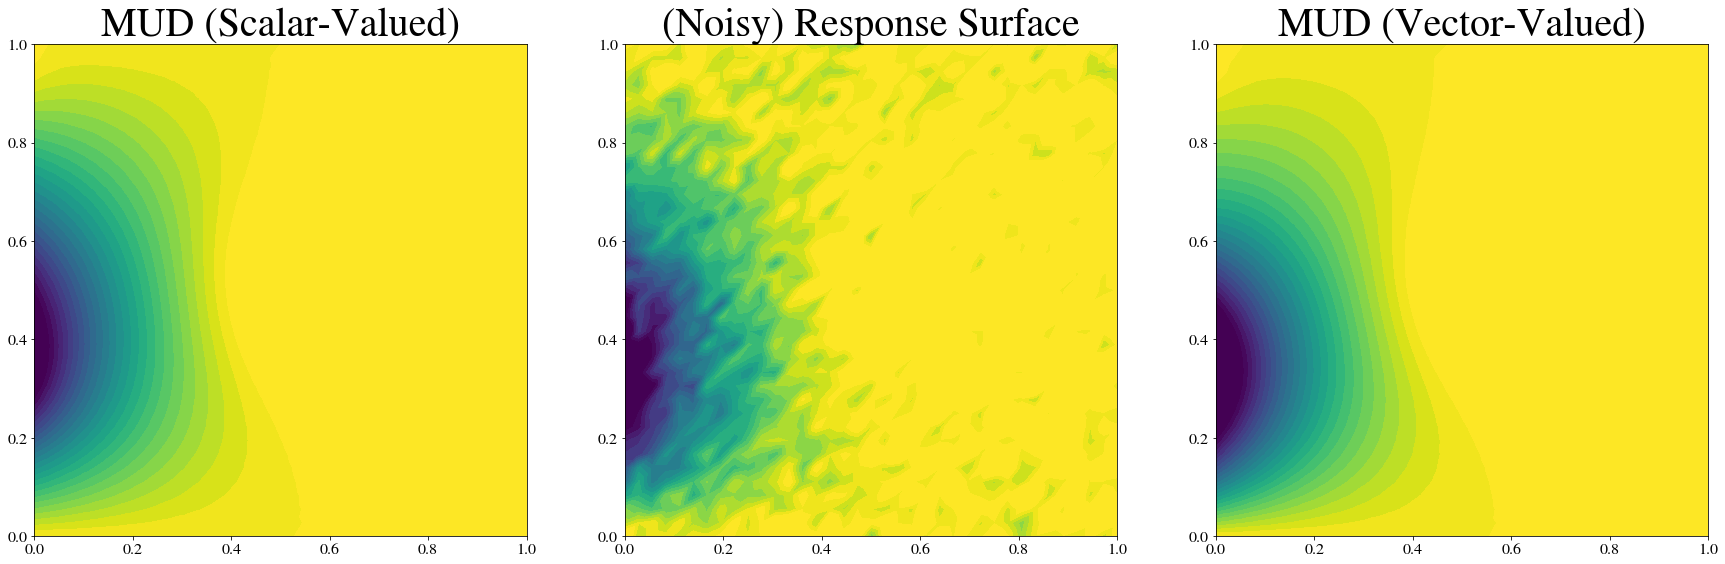
\includegraphics[width=0.95\linewidth]{figures/pde-highd/pde-highd_surf_exmud_D5-alt_m100.png}
  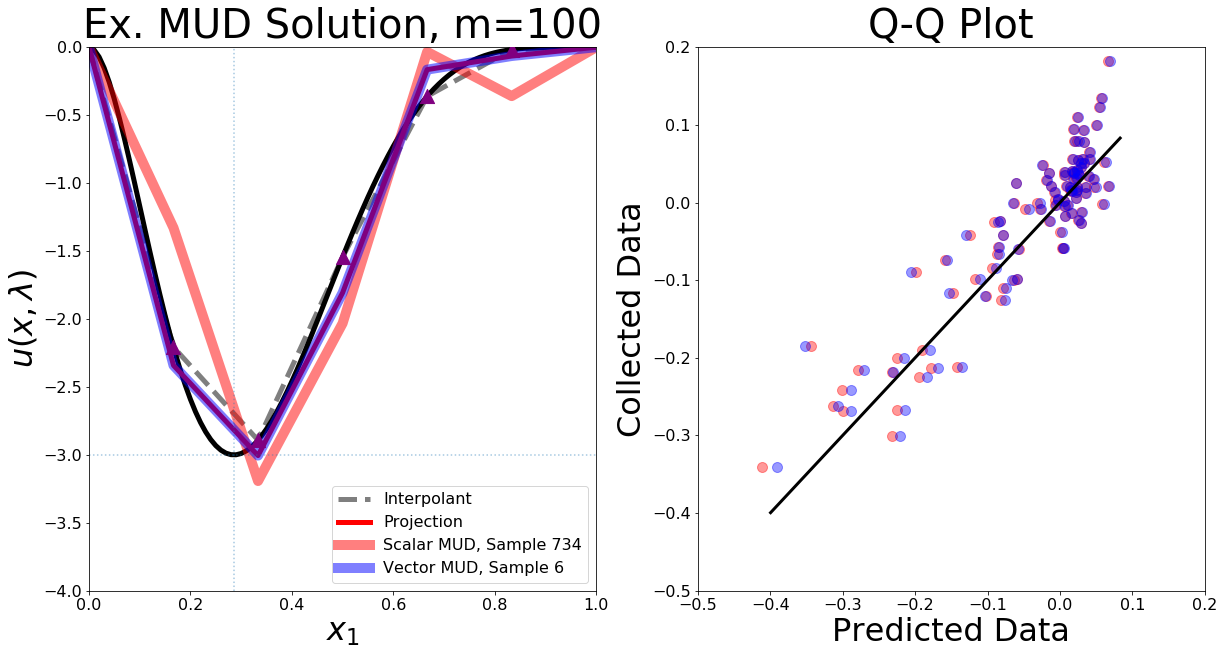
\includegraphics[width=0.9\linewidth]{figures/pde-highd/pde-highd-alt_comp_exmud_D5_m100.png}
\caption{
100 measurements for the revised five--dimensional problem yield substantially better estimates in the eyeball norm.
}
\label{fig:pde-highd-5d-alt-example}
\end{figure}


\subsubsection{Moving to Five Dimensions with more caution}

We now come to the solutions that arise from solving the same five--dimensional inverse problem of interpolating the values of $g$ through equispaced knot points, with both types of maps, in Figure~\ref{fig:pde-highd-5d-alt-mud}.
The difference in comparison to the example solutions in Fig.~\ref{fig:pde-highd-5d-mud} is stark: no longer are the solutions dramatically under-estimating the local minimum of $g$.
To the extent to which they fail to adequately to do is due to the insufficient resolution of five knot points; both scalar-- and vector--valued solutions identify the same knot as being the likely minimum, and the latter solution estimates the minima well (horizontal line drawn for reference) in the bottom-right plot.

Once again, we repeat the experiment twenty times to better understand the differences in the solutions relative to possible noise that polluted our measurements.
We are able to notice some interesting patterns by looking at the curves on the left side of Figure~\ref{fig:pde-highd-5d-alt-mud}.
First, we note that going from scalar-- to vector--valued resolves a significant amount of uncertainty in $\lambda_2$, $\lambda_3$, and $\lambda_4$, namely the QoI map appears to stop considering curves which do not have a sufficiently low minimum value.
Second, while the vector--valued MUD solution curves appear to capture the general characteristics of $g$ well, a number of them under-estimated the value at $\lambda_5$ quite severely relative to the true value (near zero), which we saw in Figure~\ref{fig:pde-highd-5d-mud} as well.

\begin{figure}[htbp]
\centering
  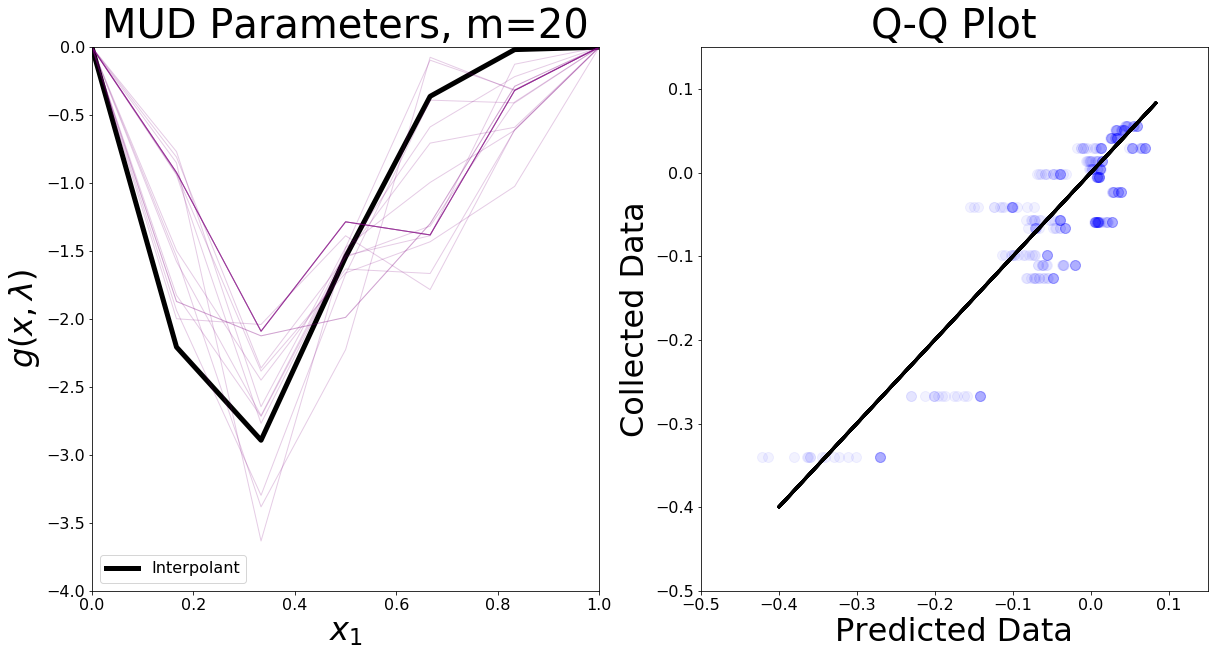
\includegraphics[width=0.95\linewidth]{figures/pde-highd/pde-highd_pair_D-alt-5-1_m20.png}
  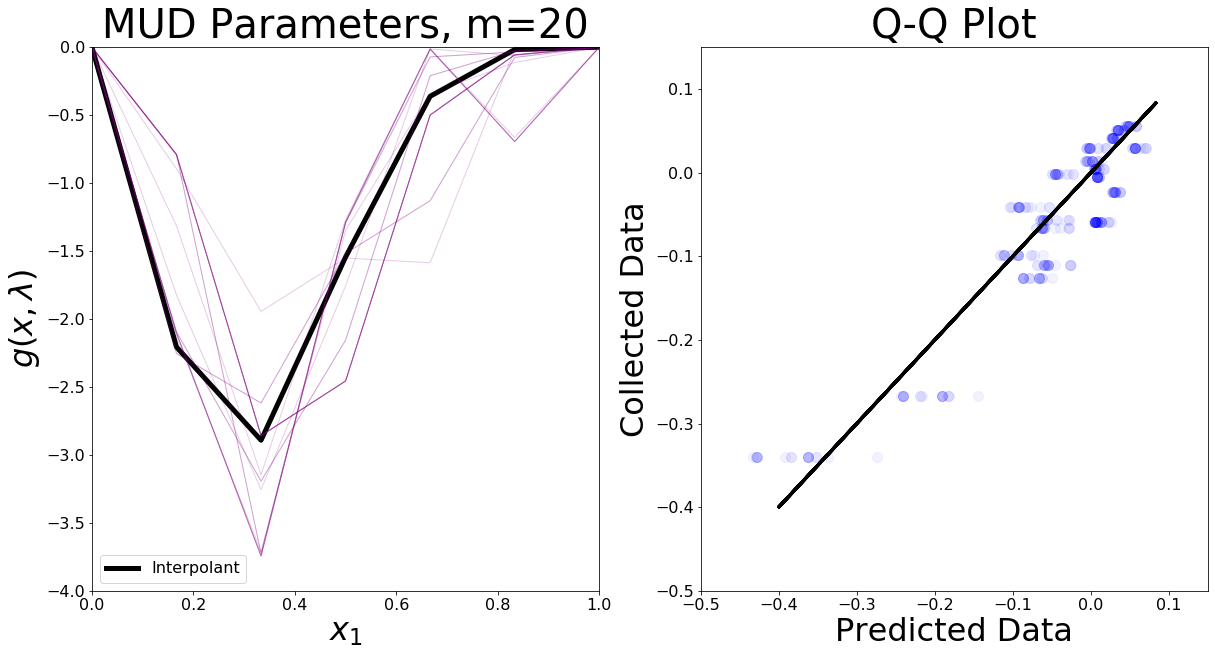
\includegraphics[width=0.95\linewidth]{figures/pde-highd/pde-highd_pair_D-alt-5-5_m20.png}
\caption{Compared to before, we're doing much better, even with less data incorporated into our QoI maps.}
\label{fig:pde-highd-5d-alt-mud-20}
\end{figure}

\begin{figure}[htbp]
\centering
  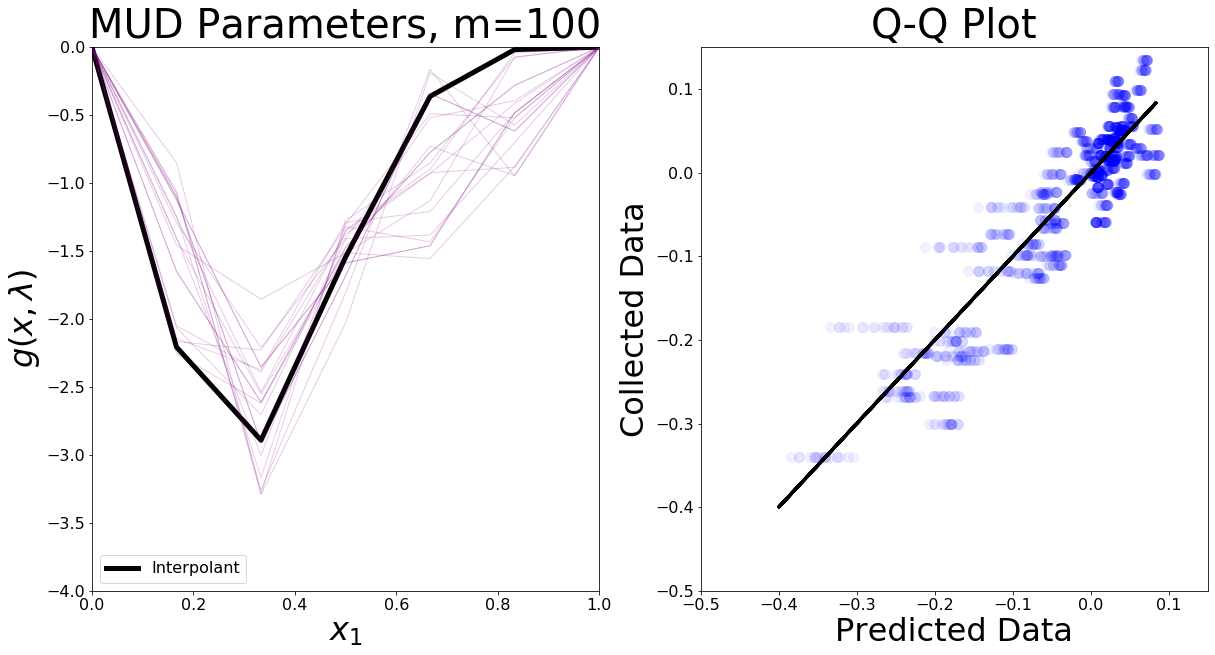
\includegraphics[width=0.95\linewidth]{figures/pde-highd/pde-highd_pair_D-alt-5-1_m100.png}
  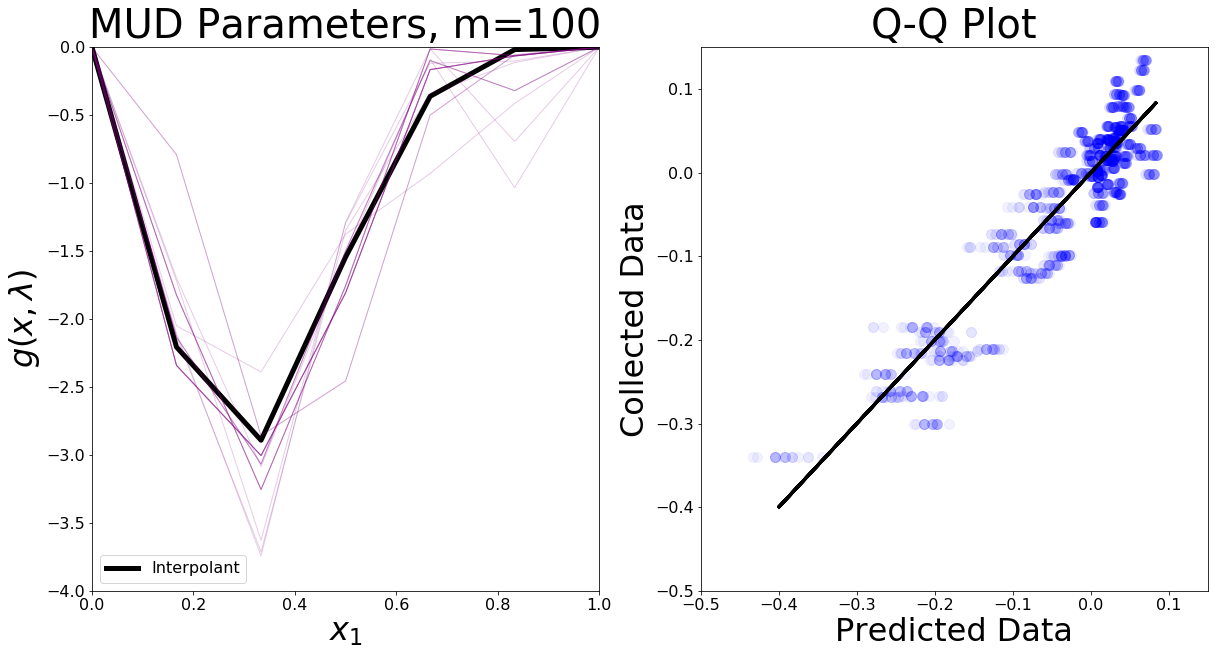
\includegraphics[width=0.95\linewidth]{figures/pde-highd/pde-highd_pair_D-alt-5-5_m100.png}
\caption{
(Top): Scalar-valued solutions for alternative approach to the five-dimensional problem.
(Bottom): Vector-valued solutions.
Because we began with a better choice of initial density, both QoI maps resolve the residuals similarly (bottom-left), and produce qualitatively similar estimates of the response surface. We attribute this to the fact that the vector--valued samples were used to bound the space, but note the direction was informed by the scalar--valued samples.
}
\label{fig:pde-highd-5d-alt-mud}
\end{figure}
\FloatBarrier


\subsubsection{Demonstration of Reduction in Uncertainty}

As a final note on this experiment, we contrast the resulting $L^2$-errors to $g$ \footnote{derived from computational approximation with the trapezoidal rule} of these MUD solutions, to the previous two examples in Figure~\ref{fig:pde-highd-5d-hist}, to show a lineage of learning, so-to-speak.
With each successive problem, our uncertainty is reduced and our MUD solutions lower in variance and increase in accuracy.
Note that they appear to be moving towards a value away from zero, which represents a fixed bias (five equispaced knots can only approximate this $g$ so well).

\begin{figure}[htbp]
\centering
  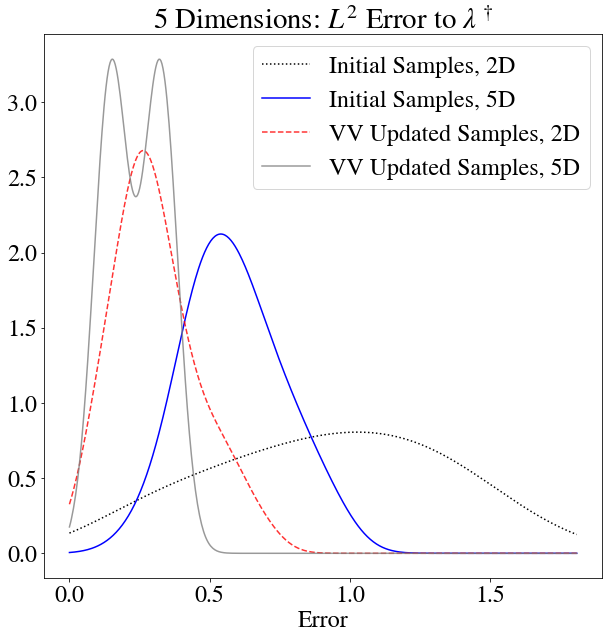
\includegraphics[width=0.675\linewidth]{figures/pde-highd/pde-highd_hist_D5_t5-0E-01}
\caption{
Comparison of the 2D initial errors to the 5D ones, as well as the reduction of uncertainty that solving a SIP problem for each provides.
}
\label{fig:pde-highd-5d-hist}
\end{figure}

\FloatBarrier


\section{Sequential Inversion}\label{sec:ch05-sequential}

The DCI framework relies on evaluating the ration function $r(\param)$ in $\dimD$--dimensional QoI space, so we turn our attention to addressing the challenges associated with the growth of this space.
As $\dimD$ increases, we must approximate a push-forward distribution with perhaps a fixed number of samples (from model evaluations) $\nsamps$, which represents a considerable source of error since the convergence rate for kernel density estimation with Gaussian kernels is $\mathcal{O} (N^{2+\dimD})$.

For example, suppose we have a time-dependent problem for which hundreds of spatial sensors are providing streams of data.
Approximating a hundred-dimensional space with $\nsamps = 1E3$ or $1E4$ samples (as we have been using for demonstrations), is wrought with problems.
However, either of these values for $\nsamps$ would be sufficient to estimate a one-dimensional distribution.
In some sense, approximating a QoI at each location over time is reasonable, but doing so for all of them simultaneously is not.
To this end, we propose to investigate an approach to solving the parameter estimation problem by performing inversion through a sequence of scalar-valued QoIs rather than employ a vector-valued approach.

We could choose any dimension below $\dimD$, but this sequential-scalar-valued approach provides a starting place and admits a simplicity in exposition.
By choosing a dimension of 1, we can focus solely on the order in which QoIs are inverted and dismiss the additional complexity of enumerating the combinations of QoI when dimensions can vary.
We also choose to use a linear map for convenience so that we can use the analytical solutions presented in the previous chapter without concern for approximation error.

With each iteration in the sequence of inverse problems, we are in-effect trying to explain measurements that constitute a single QoI at the expense of accuracy in others.
By contrast, the vector-valued approach seeks accuracy in all of the simultaneously.
This trade off is all about convenience, since 1-dimensional problems are computationally ``cheap,'' we can iterate through many more of them for the same computational cost.
Since by the time we finish iterating through all available QoI, the error in $Q^{(1)}$ may have been allowed to drift quite significantly away from its solution contour through the sequence of inverting through $Q^{(1)}, Q^{(2)}, \dots Q^{(100)}$.
To address this, we perform multiple passes through our set of QoI.
Borrowing from other sequential algorithms, these ``epochs'' will allow us to iterate until the solution stops changing by some predefined relative threshold, representing a lack of ``learning'' through continued effort.

We study the following motivating two-dimensional example with QoI defined by ten equispaced rotations of the unit vector $[0, 1]$ through the first two Euclidean quadrants.
We first plot the result of a single epoch in Fig.~\ref{fig:iterative-linear-demo}
\begin{figure}
  \centering
  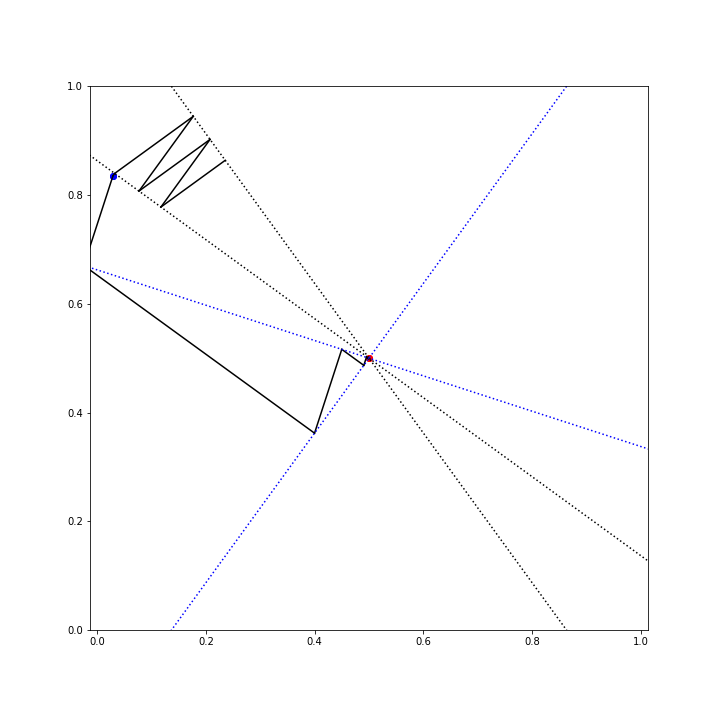
\includegraphics[width=0.475\linewidth]{examples/iterative/10D-firstepoch}
  \includegraphics[width=0.475\linewidth]{examples/iterative/10D-fewepochs}

  \caption{
  Dotted lines show the solution contours for each row of the operator $A$.
  (Left): First epoch for iterating through 10 QoI.
  (Right): Three more epochs allows our estimate to get much closer to the true value.
  }
  \label{fig:iterative-linear-demo}
\end{figure}

The spiral shape is a result of the underlying geometry of this QoI map defined by rotations. The successive rows are so similar to each other that very little is ``learned'' between each iteration; the projection doesn't cover a large distance in $\pspace$.
To drive this point home, we choose two pairs of indices from among the ten available in order to define two QoI maps, the contours for which we plot in different colors in Fig.~\ref{fig:iterative-linear-demo-pair}.
We solve a total of ten 1-D inverse problems for each of them (five epochs) to match the budget of the previous example (with ten maps and one epoch).

\begin{figure}
  \centering
  \includegraphics[width=0.475\linewidth]{examples/iterative/10D-fewepochs-pair}
  \includegraphics[width=0.475\linewidth]{examples/iterative/10D-fewepochs-pair-alt}
  \caption{
  Iterating through five epochs of two QoI, each formed by picking two of the ten available rows of $A$ at random.
  }
  \label{fig:iterative-linear-demo-pair}
\end{figure}

We observe that in Fig~\ref{fig:iterative-linear-demo-pair}, we are able to achieve much greater accuracy in estimating the true parameter value than in the case of Fig~\ref{fig:iterative-linear-demo}.
The reason for this difference is that there is more mutually distinct information between successive iterations of a pair of random rows of $A$ than there is between adjacent rows, as measured by the angle between the solution contours.

\begin{figure}
  \centering
  \includegraphics[width=0.475\linewidth]{examples/iterative/10D-firstepoch-pair-smart}
  \includegraphics[width=0.475\linewidth]{examples/iterative/10D-firstepoch-rand}
  \caption{
  If we are careful with how we construct our maps or choose our iteration strategy, we can achieve considerably more accurate solutions with the same computational cost.
  (Left): Iterating through a single epoch with a QoI formed by picking rows of $A$ which exhibit mutual orthogonality.
  (Right): Iterating through the rows of $A$ at a random order for a single epoch results in considerably more accuracy than doing so in the original order of rows of $A$.
  }
  \label{fig:iterative-linear-demo-smart}
\end{figure}

Had we chosen a pair of rows that were orthogonal, the initial mean would converge to the reference value in a single epoch (two iterations), since there is no redundancy in information whatsoever.
We show this in the left half of Figure~\ref{fig:iterative-linear-demo-smart} for two orthogonal pairs.
If we instead choose to perform no a-priori analysis of the rows of $A$ and iterated through them at random, we actually also manage to accomplish a lot more accuracy for the same amount of iterations, as seen in the right half of the figure.


\subsection{Comparisons and Convergence Results}

To make these results more concrete, we propose the following example:
We limit ourselves to solving 100 inverse problems (i.e. up to ten epochs for this map), with the \emph{only} difference between approaches being the order in which the rows of $A$ are used.
First, we use the QoI as they are presented to us, in order with respect to increased rotation angle (which defines the rows of $A$).
Next, we shuffle the rows and then perform ten epochs.
Lastly, we create an ordering based on a random shuffling of the indices representing the rows of $A$, repeated ten times, for which only a single epoch is performed.
The latter approach is similar to the second in that the same problems are solved the same number of times overall, but it lifts the restriction that a row must only be used once in each effective ``epoch''.

\begin{figure}
  \centering
  \includegraphics[width=0.95\linewidth]{examples/iterative/10D-convergence-comparison}
  \caption{
  Twenty different initial means are chosen and iterated on for three approaches.
  Individual experiments are transparent and the mean error is shown as solid lines.
  In the \emph{Ordered} approach, we iterate through the rows of $A$ as they are given to us for ten epochs.
  \emph{Shuffled QoI} refers to establishing a different random ordering of the rows of $A$ for each trial, and then
  using this ordering for ten epochs.
  Finally, in the \emph{Random QoI} approach, we choose a QoI at random for each of 100 iterations, where the ordering still ensures each row gets used ten times, representing the same overall set of inverse problems solved as the other two.
  }
  \label{fig:iterative-convergence-comparison}
\end{figure}

We see in Figure~\ref{fig:iterative-convergence-comparison} that using the rows of $A$ sequentially performs very poor, which aligns with ``spiraling'' seen in Figure~\ref{fig:iterative-linear-demo} where the first few epochs were plotted.
Shuffling the rows but requiring that every tenth iteration to use the same row (i.e., ensure same ordering for each epoch), leads to a considerable improvement by which sixteen decimal places of accuracy are achieved in under $100$ iterations.
In a few instances, the shuffled approach stumbles on an ordering that accelerates convergence, likely due to orthogonal pairs of rows in the shuffled order.
These cases exhibit the kind of behavior we saw in the left panel of Fig~\ref{fig:iterative-linear-demo-smart}; in other words, sometimes our random shuffling finds the ``smart'' rows to iterate through.
Since the ordering has no dependence on iteration number in the approach where we use random rows, we have more opportunities to find these successive orthogonal pairings, and so we see that on average, it takes fewer iterations to achieve the same accuracy.


\subsection{Iterated Solutions for a PDE Example}\label{sec:iterated-nonlinear}

Batch-updates is the connection to make here.
We are going to set up the heatrod example here but place measurement devices throughout and record the measurements at several intervals in time, the point being here that the dimension of the QoI will be higher than the input space but it's okay because we're iterating.

Some systems will be more informative early in time, others late, so the best thing to do is not really something we're going to answer, we're just going to show how this approach \emph{could} work in a situation like this where the data is streaming in over time.

\FloatBarrier

\section{Miscellaneous Extensions}


\subsection{Leveraging Data in Different Ways}\label{sec:ch05-data}
Mention the other map we can use (SSE) here.

\subsection{Addressing Model Assumptions}\label{sec:ch05-variance}
Both the maps required us to have knowledge of the variance in the measurements.
What if we got it wrong?
\emph{What if we don't know the variance? How does mis-estimating it affect our solutions?}
In this section we pose some questions and provide a brief hint at a research direction but really we do not have adequate time to flesh out the answers to these, just acknowledge that they're similar concerns shared by the Bayesians.

Multiplicative noise - handled in a straightforward way, maybe put an example here and leave it at that? Put it in appendix?


\subsection{Machine-Learning Enhancements}\label{sec:ch05-ml}

Recall that in the previous chapter we demonstrated that the MUD solution retains the accuracy of least-squares solutions while simultaneously offering the flexibility of specifying initial beliefs.
Normally in order to incorporate such beliefs, practitioners in the machine-learning field would perform Tikhonov regularization, usually with the inclusion of a hyper-parameter which scales the additional parameter-space norm in the objective function.
Mathematically, this scaling factor applied to the norm is equivalent to scaling the matrix representation of the initial (prior) covariance.
Increasing this scaling factor is interpreted as having less confidence in these initial assumptions.
Conversely, decreasing it is equivalent to putting more emphasis on the prior beliefs than the evidence provided by the data, which causes MAP solutions to drift away from the solution contour (equivalence class) to which $\lam_true$ belongs.

We summarize again that the MUD point is not impacted by such a scaling of the initial covariance, providing \emph{consistent} solutions which demonstrate levels of accuracy that MAP points only exhibit for larger values of scaling factors.
Not only is it robust to the specification of prior assumptions, but it manages to offer the flexibility of such specifications without paying the additional cost of hyper-parameter optimization that would be required for the Tikhonov solution to achieve comparable results; any choice of $\alpha$ would have sufficed.

By contrast, the Tikhonov-regularized solution selects a point that is biased in directions defined by the initial density (covariance).
The observation-consistent solution is an update to the initial mean in this same direction but always lies on the contour $Q^{-1}(\observedMean)$.
The trouble is, none of these regularization approaches actually guarantee that in under-determined problems, the unique solutions that are selected are close to $\lam_true$.

We show that regardless of how well-informed your beliefs are, the convergence rate of the MUD solutions as more data is incorporated\---either by dimension or rank)\---will match those of the Least-Squares solutions.
Moreover, the MUD solutions are not sensitive to scaling of the initial covariance (how strongly initial beliefs are held), the way that the MAP solution is.
This provides a strong motivating factor for the consideration of the observation-consistent approach within the standard set of solution methods available to scientists and modelers who seek to perform parameter-identification.
We leave the investigation of more connections to the removal of hyper-parameter estimation to future work.

[TK - can put example here about MCMC extensions, sequence of problems with resampling from updated densities. Have a notebook's worth of results with the Rosenbrock]
